\documentclass[master=cws,masteroption=ai]{kulemt}
\setup{title={Describing Images with Natural Language},
  author={Thijs Dieltjens \\ Wout Vekemans},
  promotor={Prof.\,dr.\,ir.\ Marie-Francine Moens},
  assessor={Ir.\,W. Eetveel},
  acyear={2015 -- 2016},
  assistant={Ir.\ S. Zoghbi}}
% De volgende \setup mag verwijderd worden als geen fiche gewenst is.
\setup{filingcard,
  translatedtitle={The best master thesis ever},
  udc=621.3,
  shortabstract={Hier komt een heel bondig abstract van hooguit 500
    woorden. \LaTeX\ commando's mogen hier gebruikt worden. Blanco lijnen
    (of het commando \texttt{\string\pa r}) zijn wel niet toegelaten!
    \endgraf \lipsum[2]}}
% Verwijder de "%" op de volgende lijn als je de kaft wil afdrukken
% \setup{coverpageonly}
% Verwijder de "%" op de volgende lijn als je enkel de eerste pagina's wil
% afdrukken en de rest bv. via Word aanmaken.
%\setup{frontpagesonly}

% Kies de fonts voor de gewone tekst, bv. Latin Modern
\setup{font=lm}

% Hier kun je dan nog andere pakketten laden of eigen definities voorzien
\usepackage{multirow}
\usepackage{url}
\usepackage{todonotes}
\usepackage{tikz}
\usepackage{amsmath}
\usepackage{bbm}
\usepackage{epsfig}
\usepackage[]{epstopdf}
\usepackage[export]{adjustbox}
% Tenslotte wordt hyperref gebruikt voor pdf bestanden.
% Dit mag verwijderd worden voor de af te drukken versie.
\usepackage[pdfusetitle,plainpages=false]{hyperref}

\newcommand{\myvector}[1]{$\mathbf{#1}$}

%%%%%%%
% Om wat tekst te genereren wordt hier het lipsum pakket gebruikt.
% Bij een echte masterproef heb je dit natuurlijk nooit nodig!
\IfFileExists{lipsum.sty}%
 {\usepackage{lipsum}\setlipsumdefault{11-13}}%
 {\newcommand{\lipsum}[1][11-13]{\par Hier komt wat tekst: lipsum ##1.\par}}
%%%%%%%

%\includeonly{hfdst-n}
\begin{document}

\begin{preface}
  Dit is mijn dankwoord om iedereen te danken die mij bezig gehouden heeft.
  Hierbij dank ik mijn promotor, mijn begeleider en de voltallige jury.
  Ook mijn familie heeft mij erg gesteund natuurlijk.
\end{preface}

\tableofcontents*

\begin{abstract}
  In dit \texttt{abstract} environment wordt een al dan niet uitgebreide
  samenvatting van het werk gegeven. De bedoeling is wel dat dit tot
  1~bladzijde beperkt blijft.

  \lipsum[1]
\end{abstract}

% Een lijst van figuren en tabellen is optioneel
%\listoffigures
%\listoftables
% Bij een beperkt aantal figuren en tabellen gebruik je liever het volgende:
\listoffiguresandtables
% De lijst van symbolen is eveneens optioneel.
% Deze lijst moet wel manueel aangemaakt worden, bv. als volgt:
\chapter{Lijst van afkortingen en symbolen}
\section*{Afkortingen}
\begin{flushleft}
  \renewcommand{\arraystretch}{1.1}
  \begin{tabularx}{\textwidth}{@{}p{12mm}X@{}}
  	B$n$ & Bleu $n$\\
  	BP & Brevity Penalty\\
  	CCA & Canonical Correlation Analysis \\
  	CNN & Convolutioneel Neuraal Netwerk \\
  	CV & Computer Vision \\
  	FSMN & Fast-forward Sequential Memory Neural network\\
  	gLSTM & Guided Long Short Term Memory \\
    LDA  & Latent Dirichlet Allocation \\
    LSTM & Long Short Term Memory \\
    (MS) COCO & Microsoft Common Objects in COntext dataset\\
    NLP & Natural Language Processing\\
    NP & Noun Phrase (naamwoordgroep)\\
    POS & Part of Speech (woordsoort)\\
    PP & Propositional Phrase (voorzetselgroep)\\
    RCNN & Region Convolutional Neural Network \\
    ReLu & Rectified Linear Unit\\
    RFF & Random Fourier Feature \\
    RGB & Red Green Blue\\
    RNN & Recurrent Neuraal Netwerk \\
    tf-idf & term frequentie en inverse document frequentie gewichten \\
	VDR & Visual Dependency Representation (Visuele Afhankelijkheid Representatie)\\
	VP & Verb Phrase (werkwoordgroep)\\

  \end{tabularx}
\end{flushleft}


\section*{Symbolen}
\begin{flushleft}
  \renewcommand{\arraystretch}{1.1}
  \begin{tabularx}{\textwidth}{@{}p{12mm}X@{}}
    $\theta$    & Kansverdeling van onderwerpen per document (LDA) \\
    $\phi$      & Kansverdeling van woorden per onderwerp (LDA)  \\
    $\sigma$    & Leersnelheid (learning rate) neuraal netwerk \\
    $w_{ji}$    & Woord op positie $j$ in document $i$\\
    $z_{ji}$    & Onderwerp op positie $j$ in document $i$

  \end{tabularx}
\end{flushleft}

% Nu begint de eigenlijke tekst
\mainmatter

\chapter{Inleiding}
\label{inleiding}
%In dit hoofdstuk wordt het werk ingeleid. Het doel wordt gedefinieerd en er
%wordt uitgelegd wat de te volgen weg is (beter bekend als de rode draad).
Het doel van deze masterproef is het ontwikkelen van een systeem dat in staat is om automatisch afbeeldingen te beschrijven. Dit probleem combineert twee domeinen uit de computerwetenschappen: enerzijds computervisie (CV) en anderzijds natuurlijke taalverwerking (NLP). Concreet moet het ontworpen systeem ongeziene afbeeldingen kunnen omzetten in vloeiende, grammaticaal correcte Engelstalige zinnen. Bovendien moeten deze zinnen een zo volledig mogelijke omschrijving van de afbeelding vormen. Een voorbeeld van dergelijke afbeelding samen met een automatisch gegenereerde beschrijving is te zien in figuur \ref{fig:example_img}. Het concrete doel bestaat erin een bestaand systeem uit te breiden en te verbeteren. Hoofdstuk \ref{chap:Probleembeschrijving} gaat dieper in op deze doelstelling en licht de meest frequent gebruikte datasets voor training en evaluatie van beschrijvingssystemen toe.

\begin{figure}[tb]
    \centering
    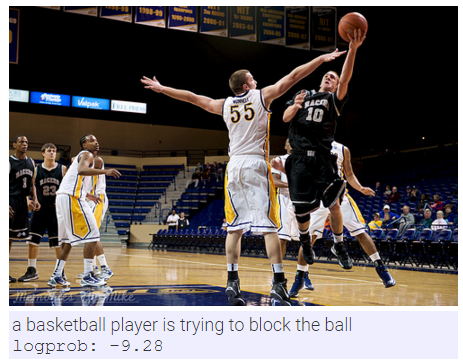
\includegraphics[width=0.65\textwidth]{Images/Results/Perfect/blocking_the_ball}
    \caption{Afbeelding met automatisch gegenereerde beschrijving}
    \label{fig:example_img}
\end{figure}

Om een beter inzicht te krijgen in het probleem en de mogelijke oplossingen, biedt hoofdstuk \ref{hoofdstuk:related} een uitgebreide literatuurstudie. Deze studie bekijkt relevante werken uit de computervisie en de natuurlijke taalverwerking. Daarnaast ligt de focus voornamelijk op recente onderzoeken die een soortgelijk doel als deze masterproef nastreven. Hieruit volgt een vergelijking van hoe deze papers afbeeldingen en zinnen voorstellen. Vervolgens onderzoekt de literatuurstudie op welke verschillende manieren deze representaties leiden tot een concreet systeem voor afbeeldingsbeschrijving.

Na de literatuurstudie volgt in hoofdstuk \ref{hst-theorie} een theoretische uitdieping van de concepten beschreven in de literatuurstudie. Een eerste sectie focust op neurale netwerken, die de basis vormen van het uiteindelijke systeem. Daarna volgt een uitdieping van twee statistische concepten die helpen bij het extraheren van zinvolle informatie uit afbeeldingen.

Hoofdstuk \ref{hst-meth} bespreekt de gebruikte methodologie om het afbeeldingsbeschrijvingsprobleem op te lossen. Een eerste sectie focust op een onderzoek (en bijhorende implementatie) uit de literatuurstudie die het basiswerk van deze masterproef vormt. Het doel van deze thesis is het verbeteren van de resultaten van dit referentiewerk. Het hoofdstuk start dan ook met een uitgebreide bespreking van het startpunt. Daarna volgt een beschrijving van eigen uitbreidingen van deze implementatie. Deze uitbreidingen behandelen nieuwe datasets, andere types neurale netwerken, verschillende vormen van extra semantische informatie en een vorm van normalisatie voor het genereren van de nieuwe zinnen. 

Om de verschillende uitbreidingen te kunnen vergelijken met het startpunt en modellen uit de literatuur, moet er een uniforme manier zijn om te evalueren. Menselijke evaluatie is hiervoor de ideale oplossing, maar dit is praktisch niet haalbaar. Om die reden bestaan er verschillende methodes om een getraind systeem te beoordelen. Hoofdstuk \ref{hoofdstuk:evaluatie} biedt een overzicht van automatische evaluatiemethodes uit de literatuur, alsook een aantal nieuwe evaluatiecriteria die de performantie van verschillende systemen vergelijken.

Hoofdstuk \ref{cha:experimenten} bevat een bespreking van de uitgevoerde experimenten. Het biedt een overzicht van de configuraties van de verschillende netwerken en hun uitbreidingen. Naast de experimenten gerelateerd aan het genereren van nieuwe zinnen, beschrijft dit hoofdstuk ook een tweede type experiment, dat twee systemen vergelijkt in hun gevoeligheid voor onzuivere datasets.

In hoofdstuk \ref{cha:resultaten} volgt een uitvoerige analyse van de resultaten van de eerder beschreven experimenten. Dit hoofdstuk bevat ook een vergelijking van de eigen systemen met de best presterende werken uit de literatuur.

Hoofdstuk \ref{besluit} besluit onze bijdrage met een overzicht van de conclusies die gemaakt zijn doorheen de masterproef.
 
%%% Local Variables:
%%% mode: latex
%%% TeX-master: "masterproef"
%%% End:

\chapter{Probleembeschrijving}
\label{chap:Probleembeschrijving}

Dit hoofdstuk beschrijft het probleem van automatische afbeeldingsbeschrijving. Een eerste sectie gaat over het concrete vraagstuk en hoe het gesitueerd is binnen de computerwetenschappen. Een tweede sectie beschrijft de meest gebruikte datasets voor het trainen en evalueren van systemen.

\section{Omschrijving en situering}
\label{sec:Omschrijving en situering}
Voor een mens is het beschrijven van een afbeelding zeer eenvoudig. Hij ziet in een oogopslag welke objecten zich op de foto bevinden, en in welke relaties ze zich verhouden. Door een aangeboren taalgevoel is het bedenken van een beschrijvende zin allesbehalve problematisch.

Afbeeldingsbeschrijving bevindt zich op het snijpunt van computer vision en natuurlijke taalverwerking, net door de combinatie van afbeeldingen en tekst. Daardoor is er nood aan een combinatie van technieken uit beide vakgebieden. Eerst moeten de verschillende objecten op de foto herkend worden. De computer moet ook een notie hebben van wat elk object net is om daarna een grammaticaal correcte, vloeiende zin te genereren. Om dit laatste te doen is het nodig dat de computer een soort van ``taalgevoel'' heeft.

Het genereren van beschrijvingen is dicht gerelateerd aan andere, eerder onderzochte problemen. Het opzoeken van afbeeldingen is hier het bekendste voorbeeld van. Op basis van een aantal sleutelwoorden, of een volledige zin, wordt een database van afbeeldingen doorzocht naar die afbeelding die het beste overeenkomt met de vraag.

Het automatisch herkennen van objecten in afbeeldingen vormt een van de meer onderzochte vraagstukken in het domein van computer vision. Zoals eerder gezegd, is er niet enkel nood aan algoritmes om vormen te detecteren in afbeeldingen, maar moet er ook een adequate labeling zijn. Een zeer gelijkaardig probleem is het classificeren van een volledige afbeelding, waarbij de hele afbeelding een label krijgt in plaats van de gedetecteerde objecten.

De concrete probleemstelling voor het vraagstuk van afbeeldingsbeschrijving is de volgende: ``Genereer een vloeiende Engelse zin die beschrijft wat er op een nooit eerder geziene foto staat''. In het vervolg van deze masterproef proberen wij dan ook een oplossing aan te reiken voor dit complexe probleem.

\section{Datasets}
\label{sec:Datasets}
Deze sectie beschrijft de drie meest gebruikte datasets voor training en evaluatie van modellen voor afbeeldingsbeschrijving: Flickr8k, Flickr30k en MS COCO.

\paragraph{Flickr8k}
\label{par:Flickr8k}
De Flickr8k dataset, zoals voorgesteld in \cite{Hodosh2013} bevat 8,092 foto's vanop \texttt{flickr.com}. De focus doorheen de afbeeldingen ligt op mensen en dieren (vooral honden) die een actie uitvoeren. De foto's zijn manueel geselecteerd om de grootst mogelijke vari\"eteit te garanderen.

De bijhorende beschrijvingen zijn manueel opgesteld door mensen met Engels als moedertaal. Een voorafgaande test van de personen die de zinnen schrijven moet de correctheid van de beschrijvingen garanderen. Eenzelfde afbeelding kan tot verschillende beschrijvingen leiden: sommige mensen focussen op de actie, anderen leggen de nadruk op de persoon die de actie uitvoert, \ldots De zinnen \texttt{A man is skiing down a hill} en \texttt{A man is going down a hill on his skis} beschrijven dezelfde foto, maar doen dit op een verschillende manier. Om deze rijkdom in taal te kunnen weergeven zijn er meerdere zinnen per afbeelding opgenomen in de dataset.

De dataset is verdeeld in drie delen, voor training, validatie en testing. De validatie- en testset bevatten elk 1000 foto's, de trainingsset bevat de overige 6092.


\paragraph{Flickr30k}
\label{par:Flickr30k}
Deze dataset \cite{Young2014} is een uitbreiding van Flickr8k. In totaal zijn er 31,783 foto's, met elk 5 beschrijvingen. Het proces dat gebruikt is om de dataset op te stellen is hetzelfde als bij Flickr8k \cite{Hodosh2013} en ook hier bestaan de test- en validatieset uit 1000 foto's, met de resterende 29,783 in de trainingsset.


\paragraph{MS COCO}
\label{par:MS COCO}
De Microsoft Common Objects in COntext dataset (MS COCO) \cite{Lin2014} staat los van de Flickr datasets en probeert een ander type van afbeelding te brengen. Ze bevat meer dan 330,000 afbeeldingen die elk vijf beschrijvingen hebben. De afbeeldingen zijn geselecteerd vanop \texttt{flickr.com}

MS COCO probeert meer te bieden dan ``standaard'' foto's. De auteurs maken een onderscheid tussen afbeeldingen van iconische objecten en iconische sc\`enes, en non-iconische afbeeldingen. Iconische afbeeldingen vormen typisch de eerste zoekresultaten bij een Google Image Search, maar ze bevatten te weinig informatie. Bijgevolg leiden ze ook tot minder interessante beschrijvingen. Non-iconische afbeeldingen brengen algemeen gezien een compositie van verschillende objecten en personen, gefotografeerd vanuit een niet-canonische hoek. MS COCO bevat voornamelijk niet-iconische afbeeldingen. Figuur \ref{fig:cocotypes} toont duidelijk het verschil tussen iconische en non-iconische afbeeldingen.

\begin{figure}[tb]
    \centering
    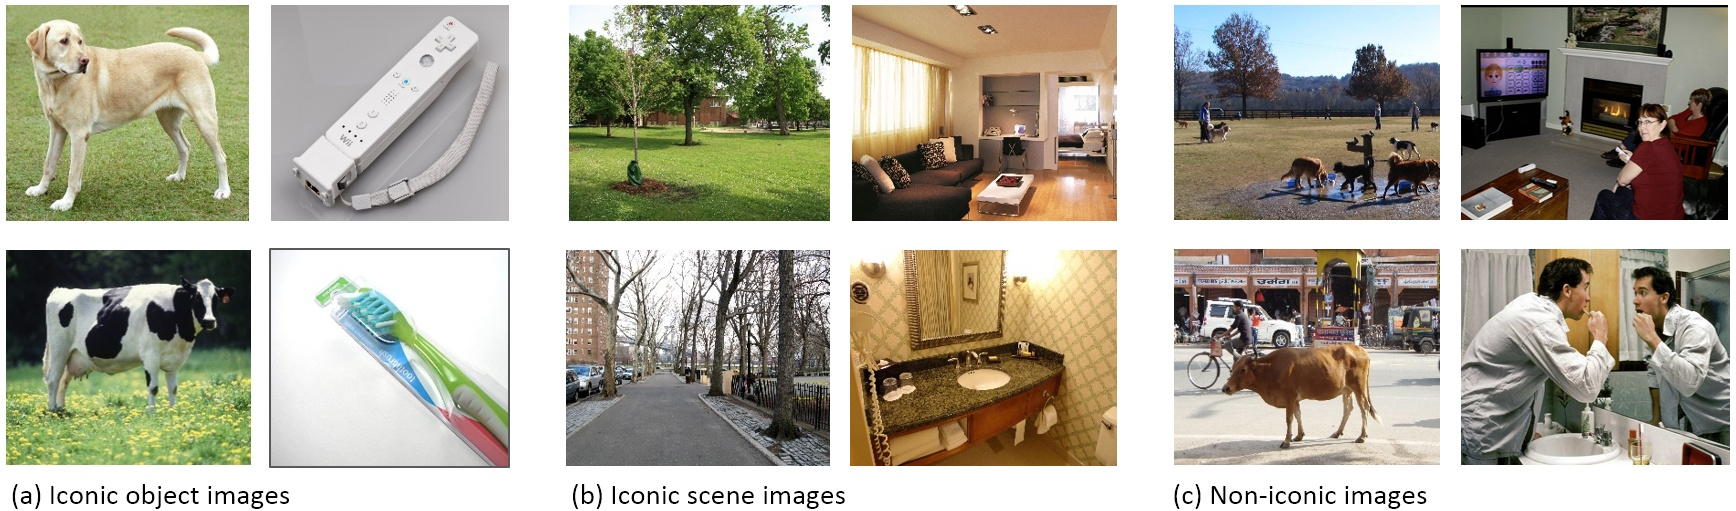
\includegraphics[width=\linewidth]{Images/iconic.jpg}
    \caption{Verschil tussen iconische en non-iconische afbeeldingen}
    \label{fig:cocotypes}
\end{figure}

Een ander belangrijk deel van de COCO dataset zijn annotaties. Oudere datasets legden de focus op classificatie, bounding boxes en segmentatie, terwijl MS COCO probeert om elk belangrijk object op de foto te annoteren. De afbeeldingen zijn gebaseerd op een lijst van object categorie\"en en zijn specifiek geselecteerd om niet-iconische sc\`enes te bevatten.

Het genereren van de beschrijvingen bij de foto's gebeurt met Amazon Mechanical Turk workers, net zoals bij de Flickr datasets. Uitgebreide instructies voor de workers garanderen dat elk belangrijk deel van de afbeelding voorkomt in de beschrijving. \cite{Rampf2015} Op figuur \ref{fig:coco_ui} is te zien op welke wijze de proefpersonen een beschrijving moesten ingeven.


\begin{figure}[tb]
    \centering
    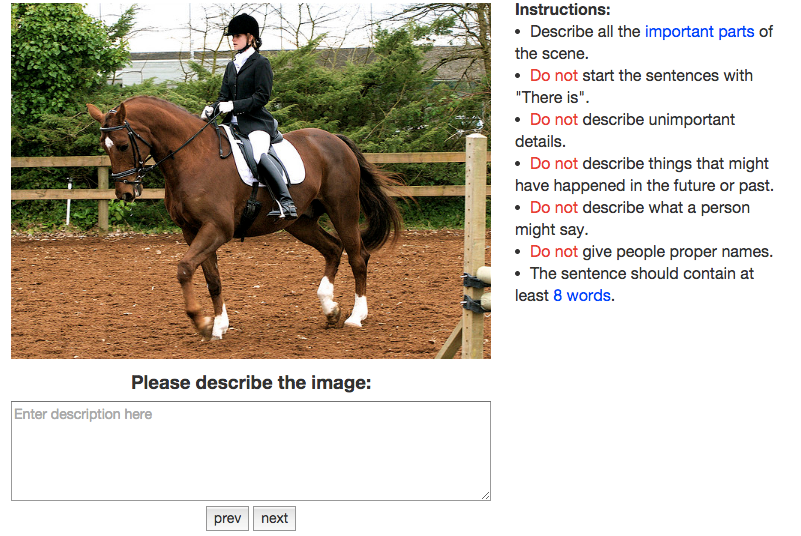
\includegraphics[width=0.8\linewidth]{Images/coco_UI.png}
    \caption{User interface voor het ingeven van afbeeldingsbeschrijvingen MS COCO}
    \label{fig:coco_ui}
\end{figure}

%%% Local Variables: 
%%% mode: latex
%%% TeX-master: "masterproef"
%%% End: 
\chapter{Gerelateerd werk}
\label{hoofdstuk:related}
Het automatisch genereren van beschrijvingen voor ongeziene afbeeldingen is een complex proces. Het combineert namelijk zowel computervisie (CV) als natuurlijke taalverwerking (NLP). Vele modellen zijn al voorgesteld die telkens elementen uit beide onderzoeksvelden combineren. 

Dit hoofdstuk begint met een vergelijking van verschillende mogelijkheden om afbeeldingen en zinnen voor te stellen. De meest relevante onderzoeken uit CV en NLP komen aan bod. Daarna volgt een samenvatting van de verschillende mogelijkheden om deze technologie\"en te integreren in \'e\'en model. 

Doorheen de jaren is deze integratie op verschillende manieren aangepakt. Het probleem van automatische afbeeldingsbeschrijving werd eerst niet beschouwd als generatieprobleem maar als opvraag- of \emph{retrievalprobleem}. Hierbij zoekt een model naar de beste zin in een bestaande verzameling van zinnen op basis van de ingevoerde foto \cite{Hodosh2013}. Nieuwere papers behandelen het probleem als een vertaalprobleem naar analogie met automatisch vertalen. Hierbij gebruikt men een codeer-decodeersysteem waarbij de afbeelding als brontaal wordt beschouwd en het Engels als doeltaal. Dit hoofdstuk biedt een overzicht van deze recentste technieken.

\section{Representatie van afbeeldingen}
Alle recente modellen gebruiken technieken uit computervisie om nuttige kenmerken af te leiden uit afbeeldingen. Kenmerken bevatten onder andere gedetecteerde acties, sc\`enes en objecten met hun attributen en relaties\cite{Bernardi}. Deze kenmerken vormen de basis voor een representatie van de afbeelding die als input dient voor het generatie- of opvraagmodel.

Eerst volgt een bespreking van technieken uit het verleden. Daarna beschrijft deze sectie Convolutionele Neurale Netwerken (CNN), die in de meer recente literatuur veelvuldig voorkomen.


\subsection{Oorspronkelijke CV modellen}
De literatuur gebruikt meerdere technieken uit computervisie om nuttige features of kenmerken af te leiden uit afbeeldingen. Kenmerken die in de vroegste papers over dit onderwerp voorkomen zijn bijvoorbeeld het type van de algemene sc\`ene, gedetecteerde objecten en attributen van deze objecten\cite{Farhadi2010,Patterson2014,Yang2011}.

Bij sc\`eneclassificatie leert een model voor ongeziene afbeeldingen een bepaalde algemene sc\`ene (bijvoorbeeld restaurant, slaapkamer, keuken) af te leiden. Ook modellen die verschillende objecten detecteren hebben hun nut. Van zulke gevonden objecten kunnen classifiers ook nog nuttige attributen zoals kleur bepalen. Om zulke afleidingen te maken, gebruiken de papers bestaande classifiers en detectoren zoals bij Felzenswalb et al.\cite{Felzenszwalb2008}, Im2Text\cite{Ordonez2011} en GIST\cite{Oliva2006}. Ee\'n of meerdere van deze features kan dan rechtstreeks de representatie vormen van een afbeelding. Daarnaast vormen deze features in een aantal werken\cite{Farhadi2010,Li2011,Mitchell2012,Yang2011} enkel de input voor abstracte afbeeldingsrepresentaties in de vorm van tupels. Deze tupels bevatten dan objecten, acties tussen objecten, sc\`enetypes en/of ruimtelijke relaties.

Een andere manier om afbeeldingen voor te stellen is het gebruik van Visual Dependency Representations (VDR) zoals voorgesteld door Elliott et al.\cite{Elliott2013}. Dit model werkt analoog aan een taalgebaseerde afhankelijkheidsgrammatica. Dit type grammatica stelt de syntactische structuur van een zin voor met woorden met daartussen binaire semantische of syntactische relaties\cite{Jurafsky:2009:SLP:1214993}. Figuur \ref{fig:dep_grammar} toont een voorbeeld van een zin ontleed met een afhankelijkheidsgrammatica. De gelabelde pijlen stellen de verschillende relaties tussen de woorden voor.

\begin{figure}[tb]
      \centering
      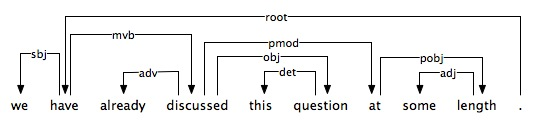
\includegraphics[width=\linewidth]{Images/dependencygrammar.jpg}
      \caption{Zin ontleed met afhankelijkheidsgrammatica\cite{GasserNotes}}
      \label{fig:dep_grammar}
  \end{figure}  

VDR's gebruiken een afhankelijkheidsgraaf om de ruimtelijke relaties tussen regio's in een foto voor te stellen. Elke relatie tussen twee objecten krijgt dan een ruimtelijke positie als label. Mogelijke relaties zijn bijvoorbeeld \texttt{op}, \texttt{boven}, \texttt{onder}, \texttt{naast}, ... Het leren van VDR's kan op basis van geannoteerde trainingsdata, automatisch met objectherkenning\cite{Elliott2015} of met nog andere informatie die in de abstracte sc\`ene zit\cite{Gilberto2015}.  

\todo[inline]{Framenet vermelden?}

\subsection{CV met neurale netwerken}
Naast deze meer traditionele manieren om informatie uit afbeeldingen af te leiden, bieden neurale netwerken een alternatieve oplossing. Voor een theoretische uitwerking van de gebruikte neurale netwerken, zie hoofdstuk \ref{hst-theorie}.

Voor de meeste taken binnen computervisie blijkt dat convolutionele neurale netwerken (CNN) beter presteren dan bovenstaande methodes.\todo{hier sta iets bij geschreven, ik denk dat het ``hoe?'' is} Deze CNN's zijn deep learning neurale netwerken met soms meer dan 15 verborgen lagen. Ze hebben minder verbindingen en parameters dan overeenkomstige feedforward neurale netwerken terwijl ze niet veel slechter presteren\cite{Krizhevsky2012a}. 
Voor verschillende CV-taken werken de huidige state-of-the-art oplossingen op basis van CNN's. Dit is onder andere het geval voor gezichtsherkenning\cite{Zhou2015}, tekenherkenning\cite{Ciresan2012} en objectherkenning\cite{Szegedy2014}.

De gebruikte CNN's binnen het automatisch beschrijven van afbeeldingen zijn getraind op ImageNet\cite{Russakovsky2014}. ImageNet is een dataset bestaande uit miljoenen afbeeldingen die gelabeld zijn binnen enkele duizenden categorie\"en. Het neuraal netwerk leert afbeeldingen correct te classificeren. Vaak gebruikte CNN modellen zijn AlexNet\cite{Krizhevsky2012a} en het recentere VGGNet\cite{Arge2015}.

Elke afbeelding dient als input voor het netwerk om zo tot een representatieve vector te komen. De meeste papers die afbeeldingen beschrijven gebruiken de gewichten van de laag voor de uiteindelijke classificatie als representatie van een afbeelding\cite{Chen2014,Karpathy2015,Mao2014a,Google}. Aandachtsgebaseerde oplossingen\cite{Jin2015,Xu2015} gebruiken ook de output van lagere convolutionele lagen als extra informatie.

Regionale CNN's vormen een variatie op CNN die een afbeelding opdeelt in verschillende interessante regio's. Hiermee is het mogelijk om voor elke regio een representatie te maken\cite{Karpathy2015,Mitchell2015}. 

\section{Representatie van zinnen}
Het is niet eenvoudig om rechtstreeks met zinnen als een geheel te werken. Daarom zijn er verschillende alternatieven onderzocht om een zin voor te stellen.
De meeste modellen vertrekken van een vectorrepresentatie voor individuele woorden. In de literatuur zijn er verschillende manieren beschreven om woordrepresentaties samen te voegen tot een representatie van een zin.

\subsection{Voorstellen van woorden}
 Het voorstellen van woorden met een vector vergemakkelijkt de verdere verwerking en kan bovendien ook semantische informatie bevatten.

 Een eerste mogelijke voorstelling is een one-hot codering waarin een vector met als grootte het aantal woorden in het vocabularium elk woord voorstelt. Deze vector is volledig nul behalve op \'e\'en rij die overeenkomt met het woord. Het is mogelijk om deze representatie verder uit breiden door vermenigvuldiging met een gewichtsmatrix. Deze matrix transformeert de one-hotvectoren naar een andere vector. Training kan zorgen voor aanpassingen aan deze gewichtsmatrix om zo ook de semantische informatie van de woorden te leren. Deze gewichtsmatrix kan willekeurig worden ge\"initialiseerd of eerst trainen op bestaande corpora\cite{Lebret2013,Mao2014a,Google}. Daarna kunnen de gekende woorden en zinnen uit de dataset de gewichten nog verfijnen.  

 Een andere mogelijkheid is om bestaande word embeddings te gebruiken zoals \texttt{word2vec}. Dat algoritme projecteert elk woord op een vooraf geleerde vector en heeft bovendien enkele mooie eigenschappen. Zo projecteert het semantisch gelijkaardige woorden op nabijgelegen posities in de vectorruimte\cite{Mikolov2013}. Deze voorgedefin\"ieerde vectoren hebben als nadeel dat niet voor elk woord uit de beschrijvingen een vector representatie beschikbaar is. Het is wel mogelijk om zelf de vectorrepresentaties te leren op basis van de gebruikte dataset zoals beschreven in de paper.

 De meeste werken in de literatuur rapporteren dat one-hotcodering in combinatie met een te leren gewichtsmatrix gelijkaardige en snellere resultaten oplevert. Daarnaast hebben sommige semantisch gelijkaardige woorden zoals kleuren gelijkaardige vectoren bij gebruik van het \texttt{word2vec} algoritme, terwijl kleuren in een afbeelding toch uitgesproken verschillend zijn. Hierdoor zal een systeem dat \texttt{word2vec} woordvectoren gebruikt, waarschijnlijk slecht presteren in het herkennen van kleuren\cite{Karpathy2015}.
 
\subsection{Voorstellen van zinnen}
 Verschillende mogelijkheden bestaan om de zinnen voor te stellen wanneer de woordvectoren gekend zijn. Een eerste mogelijkheid gebruikt een afhankelijkheidsparser en stelt de zinnen voor als een volledige afhankelijkheidsboom\cite{Socher2014}. Karpathy\cite{Karpathy2014} gebruikt ook een afhankelijkheidsparser, maar haalt hier een verzameling van triplets uit. Dergelijke triplets bestaan uit twee woorden uit de zin en hun onderlinge relatie. Figuur \ref{fig:deprelations} toont een voorbeeldzin met de bijhorende triplets. Het eerste element van de triplet is het type van de relatie.

 \begin{figure}[tb]
     \centering
     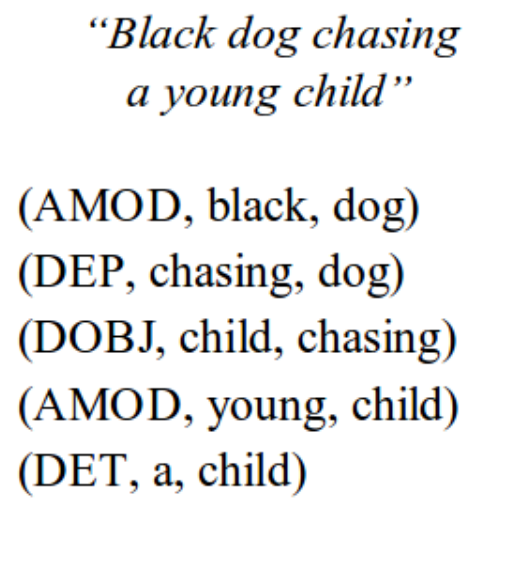
\includegraphics[width=0.35\textwidth]{Images/dep_relations}
     \caption{Zin met ontlede afhankelijkheidstriplets\cite{Karpathy2014}}
     \label{fig:deprelations}
 \end{figure}

 Een volgende optie telt de woordvectoren van een zin op\cite{Lebret2013}  Hierdoor gaat informatie uit de woordvolgorde wel verloren. Le en Mikolov\cite{Le2014a} bieden een oplossing voor het verloren gaan van woordvolgorde. Zij trainen een model om representaties te maken van stukken tekst met variabele lengte. Hun algoritme kan zowel zinnen als paragrafen en volledige teksten voorstellen.

 Een vaak gebruikt taalmodel in de meer recente NLP-literatuur is een Recurrent Neuraal Netwerk (RNN)\cite{Mikolov2010}. Dit is een neuraal netwerk dat goed overweg kan met sequenti\"ele data zoals taal. Kiros et al.\cite{Kiros2013} combineren de verborgen lagen van een RNN met extra informatie (zoals POS-tags) om tot een representatie van de zin te komen. De meer recente modellen stellen een zin voor als de sequentie van de woordvectoren in die zin. Zo kan het RNN de taal leren door elke zin woord per woord in het netwerk in te voeren.
 
\section{Van afbeeldingsrepresentaties naar beschrijvingen}
Er zijn verschillende methodes om vanuit de representaties van de afbeelding en bijbehorende referentiezinnen een model te trainen dat in staat is om ongeziene afbeeldingen om te zetten in correcte beschrijvingen. 
De meeste modellen trainen met als doel het verschil tussen de gegenereerde omschrijving en de correcte omschrijving uit de trainingsverzameling te minimaliseren.

\subsection{Dichtstbijzijnde afbeelding}
De eenvoudigste aanpak zoekt naar de meest gelijkaardige afbeelding in de trainingsverzameling en geeft \'e\'en van haar beschrijvingen terug als resultaat(Nearest Neighbour)\cite{Devlin2015a}. Een gelijkaardigheidsmetriek zoals de cosinusgelijkenis tussen de afbeeldingsrepresentaties evalueert de gelijkaardigheid van twee representaties.

Een uitbreiding op deze aanpak zoekt naar de verzameling van de meest gelijkaardige afbeeldingen in de trainingsverzameling. Vervolgens cre\"eert een model een rangorde op basis van extra visuele of tekstuele informatie. De referentiezin van de hoogst scorende afbeelding is dan het resultaat\cite{Devlin2015a,Hodosh2013,Oliva2006,Ordonez2011}. 
Deze modellen hebben als nadeel dat ze nooit resulteren in een zin die niet in de trainingsverzameling zit.

Een variatie hierop gebruikt een afbeeldingsvoorstelling met gedetecteerde objecten. Dit systeem zoekt naar de beschrijving van visueel gelijkaardige objecten in de vorm van zinsfragmenten (frases)\cite{Gupta2012,Kuznetsova2012}. Met de verzamelde fragmenten zoekt het systeem dan de meest waarschijnlijke nieuwe zin op basis van het type van de fragmenten. Deze types bestaan uit naamwoordsgroep (NP), werkwoordsgroep (VP) en voorzetselgroep (PP). De samenstelling van een nieuwe zin gebeurt dus op basis van zinsdelen die objecten gelijkaardig aan die op de foto beschrijven. De auteurs defin\"ieren meerdere beperkingen op de gegeneerde zinnen om het aantal mogelijkheden te verkleinen.

Een andere variatie op Nearest Neighbour geeft de zinnen, samen met de dichtstbijzijnde afbeelding, als input aan een tweede model. Dit model vormt deze informatie dan om tot een nieuwe zin. Zo beschouwen Mason et al.\cite{Mason2014} het genereren van beschrijvingen als een samenvattingsprobleem en gebruiken ze de beschrijvingen van gelijkaardige afbeeldingen als extra input. Analoog verkrijgen Jia et al.\cite{Fernando2015} verbeteringen op bestaande modellen door het toevoegen van extra semantische informatie zoals beschrijvingen van gelijkaardige afbeeldingen op basis van Canonical Correlation Analysis (CCA).
 
\subsection{Multimodale modellen}
Enkele werken proberen een gemeenschappelijke ruimte tussen zinnen en afbeeldingen te leren zodat het mogelijk is om de representatie van zinnen zowel als afbeeldingen op dezelfde ruimte te projecteren. Dit laat toe om afbeeldingen en zinnen rechtstreeks te vergelijken met een afstandsmaat zoals bijvoorbeeld de cosinusgelijkenis. Dit is zeer nuttig voor onder andere het opvragen van afbeeldingen met een ongeziene query en zinnen met een ongeziene afbeelding. Het leren van multimodale modellen kan onder andere met Canonical Correlation Analysis (CCA)\cite{Hodosh2013} en neurale netwerken\cite{Mao2014,Karpathy2014,Kiros2013}. 

\subsection{Sjabloongebaseerd}
Een volgende aanpak baseert zich op sjablonen om zinnen te genereren. Op basis van de gebruikte afbeeldingsvoorstelling vult een algoritme een voorgedefinieerd sjabloon in\cite{Yang2011}. Hiervoor is het dikwijls nodig om bijkomende complexe modellen te trainen\cite{Elliott2013}. Het nadeel van deze methode is dat de gegenereerde zinnen wel syntactisch correct zijn, maar dikwijls onnatuurlijk aanvoelen voor mensen. Om deze methode te verbeteren kunnen gegenereerde of vooraf gekende zinsfragmenten helpen bij het hercombineren van fragmenten\cite{Mitchell2012,Kuznetsova2012}. Daarnaast kan een algoritme een aantal gegenereerde zinnen sorteren op basis van verschillende factoren en zo de beste zin eruit halen. \todo{voorbeeld van deze factoren}

\subsection{Neurale netwerken}
De meest recente en best scorende modellen gebruiken neurale netwerken als taalmodel voor het genereren van beschrijvingen. Deze taalmodellen zijn in staat om compleet nieuwe, vlotte en natuurlijk aanvoelende zinnen te produceren. Vooral Recurrente Neurale Netwerken (RNN)\cite{Mikolov2010} winnen in de literatuur aan populariteit als taalmodel. RNN's zijn in staat om sequenti\"ele data te genereren op basis van een zekere input. LSTM's (Long Short Term Memory)\cite{SeppHochreiter1997} vormen een uitbreiding op de RNN's en onthouden informatie op lange termijn met behulp van een geheugencel.

Beide modellen verwachten een sequentie van woordrepresentaties als input, maar kunnen ook uitgebreid worden met extra informatie als invoer. Zo gebruiken meerdere werken de afbeelding als eerste invoer. Een andere toevoeging cre\"eert een multimodale ruimte tussen afbeeldingen en zinnen\cite{Kiros2014,Socher2014}. Xu et al.\cite{Xu2015} voegen een ``aandachtsvector'' toe die aangeeft waar in de afbeelding het systeem moet focussen. Het is ook mogelijk om een combinatie van verschillende technieken te gebruiken, zoals het leren van een ``sc\`enevector'' in combinatie met een aandachtsgebaseerd systeem\cite{Jin2015}. Jia et al. experimenteren met verschillende mogelijkheden om extra informatie toe te voegen, zoals CCA-projecties van afbeeldingen, of de afbeelding zelf\cite{Fernando2015}.

Een eerste verzameling van modellen met neurale netwerken volgt het codeer-decodeerprincipe uit de automatische vertaling\cite{Kiros2014}. De codeercomponent transformeert een afbeelding naar een nieuwe (multimodale) representatie. De decodeercomponent vertaalt vervolgens deze multimodale representatie naar een zin in natuurlijke taal. Door het multimodale karakter van deze modellen is het opvragen van afbeeldingen en zinnen ook mogelijk. Dit opvragen gebeurt door middel van projectie van een nieuwe afbeelding of zin in de multimodale ruimte. Een vergelijking van deze projectie met de zinnen of afbeeldingen uit de trainingsverzameling leidt tot een rangschikking van de trainingsvoorbeelden. Er bestaan zowel codeer-decodeer modellen met LSTM's\cite{Kiros2014} als met RNN's\cite{Karpathy2014,Mao2014a}.

Een tweede categorie gebruikt zowel de afbeeldingsrepresentatie als de sequentie van 
woordrepresentaties als input bij het trainen van het netwerk. Op basis van een trainingsafbeelding probeert het netwerk het eerste woord uit de zin te voorspellen. Deze voorspelling dient dan, al dan niet samen met de afbeelding, als input voor de voorspelling van het volgende woord. Terugpropagatie van de fout op de gegenereerde woorden doorheen het netwerk zorgt voor de juiste wijzigingen aan de gewichten. Op deze manier leert het netwerk om op basis van een ongeziene afbeelding de juiste sequentie van woorden te genereren. Ook hier bestaan er modellen met LSTM's\cite{Donahue2015,Google} en RNN's\cite{Karpathy2015}. \todo{meer papers toevoegen}

Het trainen van deze netwerken gebeurt doorgaans met terugpropagatie doorheen het netwerk. Het is mogelijk om de fouten ook verder door te propageren naar de gewichtsvectoren van de woordrepresentaties of naar de gewichten van een CNN. Die methode optimaliseert op die manier alle gewichten op de dataset, maar kan computationeel kostelijk zijn.

Alle neurale netwerken gebruikt in deze thesis hebben een ``softmax'' als laatste laag. Deze laag zorgt ervoor dat het netwerk een kansverdeling genereert voor het volgende woord. Het meest waarschijnlijke woord heeft dan de hoogste kans.
Het selecteren van het woord voor de generatie kan gebeuren door het samplen van deze verdeling, of door het gebruik van een zoekalgoritme zoals beam search, om zo de meest waarschijnlijke beschrijving te benaderen. Een specifiek stopwoord kenmerkt zowel het begin als het einde van de zin.

\subsection{Statistische taalmodellen}
Naast de neurale netwerken behoren ook de statistische taalmodellen tot de beter scorende modellen. Deze modellen proberen op basis van entropie een taal zo goed mogelijk te beschrijven. Entropie is een maat voor informatie en heeft verschillende doeleinden binnen het domein van NLP. 

Concreet stelt de entropie $H$ de hoeveelheid informatie voor die in een willekeurige variabele $X$ zit. $X$ is typisch de voorspelde variabele. Bij het afbeeldingsbeschrijvingsprobleem zijn dit typisch woorden of zinnen. Het domein van deze variabele is $\chi$. De entropie van $X$ is te berekenen met formule \eqref{entropy}, waarbij $p(x)$ de kans voorstelt dat $X$ waarde $x$ heeft\cite{Jurafsky:2009:SLP:1214993}. 

\begin{equation}
     H(X) = -\sum_{x \in \chi}p(x)\log_2p(x)
     \label{entropy}
 \end{equation} 

Entropie-gebaseerde modellen modelleren de kennis die zeker is en ze beschouwen onzekerheden als uniform. Als een woord vijf mogelijke vertalingen heeft, waar het systeem verder niets over weet, heeft elke vertaling een kans van $\frac{1}{5}$. Als het systeem uit observatie weet dat in 50 \% van de gevallen een van de eerste 2 vertalingen is, hebben deze twee vertalingen een waarschijnlijkheid van $\frac{1}{4}$. De andere drie vertalingen, waarover het systeem onzeker is, hebben een waarschijnlijkheid van $\frac{1}{6}$, wat neerkomt op een uniforme kansverdeling binnen de beperkingen die uit de observaties voortkomen. In andere modellen kunnen deze beperkingen voortkomen uit sjablonen, het al dan niet observeren van bepaalde woordsequenties, \ldots \cite{Berger1996}

Zo leren Mitchell et al.\cite{Mitchell2015} om een lijst met waarschijnlijke woorden uit de afbeeldingsrepresentatie te extraheren en combineren ze deze met een uitgebreid taalmodel. Dit taalmodel leert de verschillende kansen op basis van de beschrijvingen in de trainingsdata. Tijdens het leerproces probeert het algoritme de entropie te maximaliseren. In een volgende stap van hun systeem zoeken ze de zinnen die het meest waarschijnlijk zijn, gegeven de woorden die herkend zijn in de afbeelding. Vervolgens sorteren ze de gegeneerde zinnen op basis van een aantal additionele kenmerken. Dit model is net als de modellen met neurale netwerken in staat om nieuwe en vlotte zinnen te vormen. De prestatie is gelijkaardig aan die van de neurale netwerken.

Lebret\cite{Lebret2015} toont bovendien aan dat een nog eenvoudiger taalmodel toch relatief goede resultaten kan bekomen. Dit model extraheert alle zinsfragmenten (frases) uit de trainingsdata en leert daarmee een eenvoudig 3-gram taalmodel. Voor ongeziene afbeeldingen bepaalt het model de best overeenkomende zinsfragmenten en probeert hiermee zinnen te maken. In tegenstelling tot alle voorgaande modellen gebeurt training van deze multimodale transformatie met negatieve sampling. Hierbij leert het model een juiste referentiezin te onderscheiden in een lijst die ook willekeurig gekozen zinnen bevat. Ook hier gebeurt er aan het einde nog een hersortering van de gegenereerde zinnen op basis van de overeenstemming met de afbeelding.

\subsection{Aandachtsgebaseerde modellen}
State-of-the-art modellen uit het automatisch vertalen gebruiken mechanismes die aandachtsgebaseerd zijn. Concreet betekent dit dat het decodeeralgoritme zelf beslist welke stukken uit de zin meer aandacht vereisen.
In de setting van het beschrijven van afbeeldingen komt dit neer op een mechanisme dat aangeeft welke regio's in de afbeelding belangrijk zijn. In de decoder zorgt dit aandachtsmechanisme voor een extra contextvector als input voor een neuraal netwerk. 

Deze aandachtsvector kan zowel ``hard'' als ``zacht'' zijn. ``Harde'' aandacht is een stochastisch principe dat de aandachtslocatie beschouwt als een latente variabele. Tijdens elke stap samplet\todo{Nederlands woord?} het algoritme \'e\'en locatie om de aandacht op te vestigen tijdens het genereren van het volgende woord. ``Zachte'' aandachtsmethodes werken deterministisch, waardoor er geen nood is om elke stap een sample-operatie uit te voeren. Een differentieerbare functie bepaalt de aandachtslocatie tijdens elke stap van het trainingsproces. Door de differentieerbaarheid is het netwerk dat de aandachtsvector berekent eenvoudig te trainen met behulp van terugpropagatie.

Aandachtsmodellen geven bovendien een mooie visuele voorstelling van waar het model bepaalde woorden ``ziet'' (figuur \ref{fig:attention-example}). Binnen het automatisch beschrijven van afbeeldingen bereiken deze aandachtsgebaseerde modellen voorlopig de beste resultaten\cite{Jin2015,Xu2015}.

\begin{figure}[tb]
	\centering
	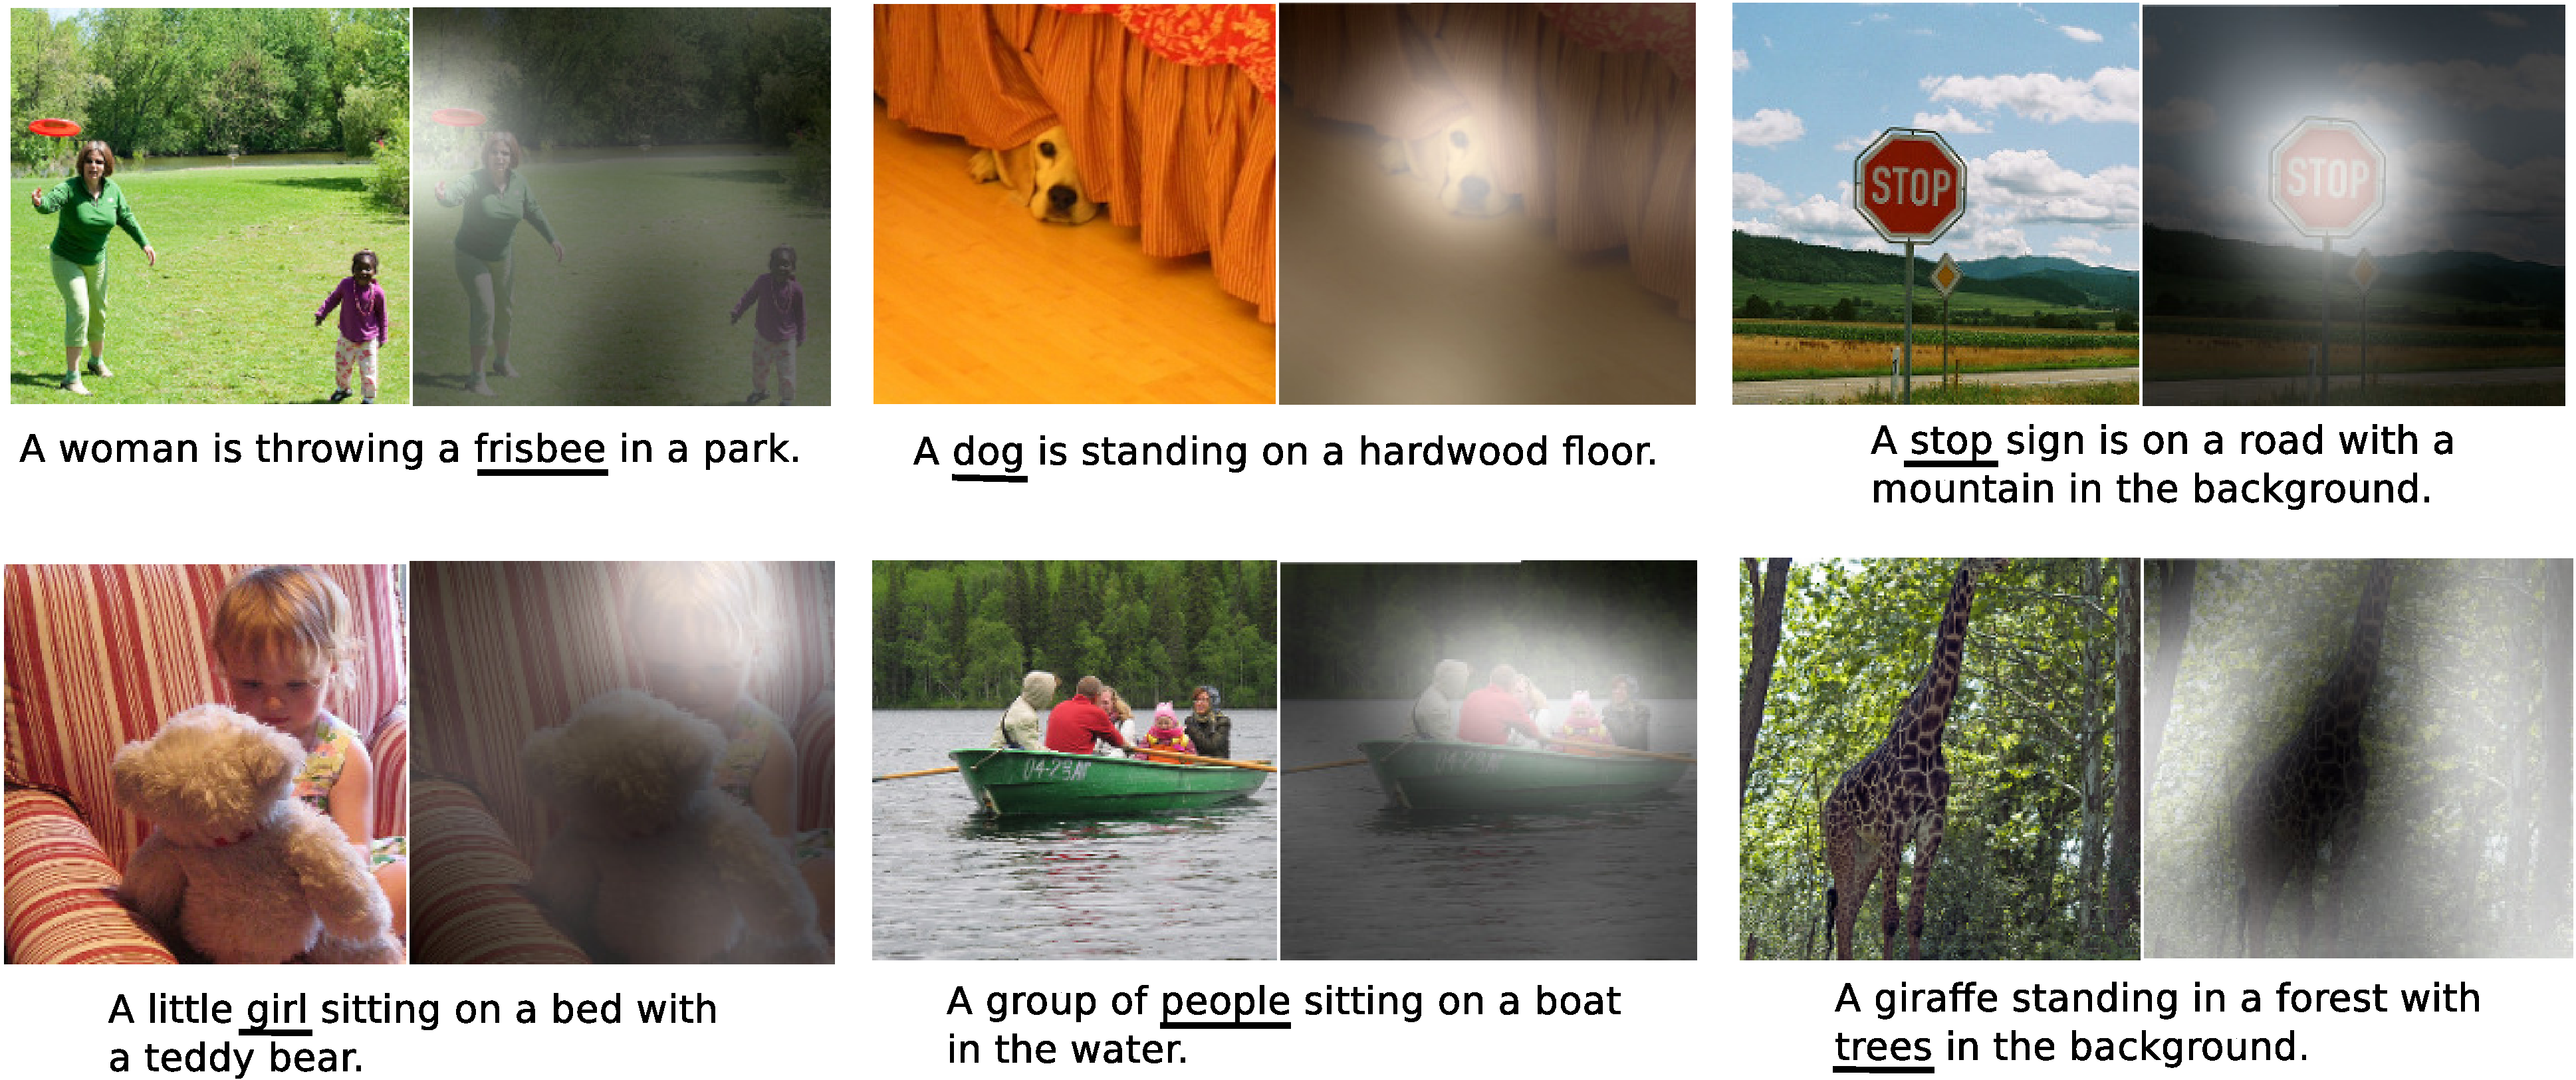
\includegraphics[width=\linewidth]{Images/good_Xu.pdf}
	\caption[Voorbeelden van aandacht op correcte regio.]{Voorbeelden van aandacht op correcte regio. (Wit in de afbeelding is de gefocuste regio, onderlijnde tekst is het overeenkomstige woord)\cite{Xu2015}}
	\label{fig:attention-example}
\end{figure}


\section{Besluit}
%%% Local Variables: 
%%% mode: latex
%%% TeX-master: "masterproef"
%%% End: 
\chapter{Theoretische Achtergrond}
\label{hst-theorie}
Dit hoofdstuk bevat de theoretische concepten die nodig zijn om de gebruikte aanpak zo goed mogelijk te begrijpen. Het bevat een beschrijving van de gebruikte neurale netwerken en van een aantal concepten uit de statistiek.

\section{Neurale Netwerken}
Algemeen gesproken dient een neuraal netwerk als een simulatie van menselijke hersenen. De structuur van een neuraal netwerk probeert de werking van de neuronen en synapsen in het menselijke brein na te bootsen. Neuronen zijn de primitieve eenheden van het menselijke zenuwstelsel. Ze staan in verbinding met elkaar en communiceren met elkaar door middel van elektrische potentiaal. Afhankelijk van de aan- of afwezigheid van potentiaal over de inkomende verbindingen stuurt een neuron al dan niet een signaal door naar het volgende neuron. Deze eenheden zijn zeer makkelijk softwarematig te simuleren.
Elk artificieel neuraal netwerk heeft een trainingsfase nodig waarin het de juiste gewichten leert. Na deze training kan het netwerk ongeziene input omvormen tot de juiste output.


Deze sectie geeft een inleiding tot de gebruikte neurale netwerken. Een eerste deel handelt over het eenvoudigste type neuraal netwerk (feedforward), dat de basis vormt voor een aantal gebruikte varianten. Daarna volgt een toelichting van enkele meer complexe netwerken: recurrente en convolutionele neurale netwerken, alsook Long Short Term Memory netwerken.

\subsection{Feed Forward Neurale Netwerken}
\paragraph{Perceptron} % (fold)
\label{par:perceptron}

Om een feedforward neuraal netwerk te begrijpen is het concept perceptron nodig. Dit is een netwerk bestaande uit een of meer neuronen, met een of meerdere inputs ($x_i$). De output $y$ van een neuron is een gewogen som van alle inputs met gewichten $w_i$, al dan niet gewijzigd met een transferfunctie $f$ (formule \ref{formule:neuron}). Typische voorbeelden van transferfuncties zijn de logistische functie en de hyperbolische tangensfunctie.

\begin{equation}
    y = f(\sum\limits_{i=1}^{n}w_i x_i)
    \label{formule:neuron}
\end{equation}

Het is ook mogelijk om een perceptron met meerdere outputs te gebruiken. Hierbij heeft elke input \'e\'en gewicht per output en kan elke output een verschillende transferfunctie hebben. Figuur \ref{fig:perceptron} toont een perceptron met vijf inputs en drie outputs. Deze architectuur komt exact overeen met drie aparte neuronen die allemaal dezelfde inputs krijgen, maar elk verschillende gewichten en een verschillende transferfunctie $f_i$ gebruiken.

\begin{figure}[ht]
\def\layersep{2.5cm}
\centering
\begin{tikzpicture}[shorten >=1pt,->,draw=black!50, node distance=\layersep]
    \tikzstyle{every pin edge}=[<-,shorten <=1pt]
    \tikzstyle{neuron}=[circle,fill=black!100,minimum size=17pt,inner sep=0pt]
    \tikzstyle{input neuron}=[neuron, fill=lime!65];
    \tikzstyle{output neuron}=[neuron, fill=red!65];
    \tikzstyle{annot} = [text width=4em, text centered]

    %input neurons
    \foreach \name / \y in {1,...,5}
        \path[yshift=0.5cm]
            node[input neuron] (I-\name) at (0,-\y cm){};

    %output neurons
    \foreach \name / \y in {1,...,3}
        \node[output neuron] (O-\name) at (\layersep,-\y-0.5) {$f_{\name}$};

    %links
    \foreach \source in {1,...,5}
        \foreach \dest in {1,...,3}
            \path (I-\source) edge (O-\dest);

    % Annotate the layers
    \node[annot,above of=I-1, node distance=1cm] (i1) {Input};
    \node[annot,right of=i1] (hl2) {Output};
\end{tikzpicture}
\caption{Perceptron met vijf inputs en drie outputs}
\label{fig:perceptron}
\end{figure}


\paragraph{Feedforward Netwerk}
\label{par:concept}
Een feedforward neuraal netwerk is een van de eenvoudigste neurale netwerken. Het is een perceptron met \'e\'en of meer verborgen lagen tussen input en output. De outputs van elke laag worden enkel doorgegeven aan de volgende laag, er zijn dus geen cycli in het netwerk (zie figuur \ref{fig:ffnn}). Elke pijl op de figuur vertegenwoordigt een vermenigvuldiging met een bepaald gewicht. Het is voor elke knoop in het netwerk ook mogelijk om een transferfunctie te gebruiken alvorens de waarde door te sturen naar de volgende laag. Hier is het ook mogelijk om een outputlaag te gebruiken met meerdere knopen, wat neerkomt op een parallelle uitvoering van meerdere netwerken met een enkele output.\cite{Bishop:1995:NNP:525960} Daarnaast hoeft een knoop niet alle outputs van een vorige laag te gebruiken. Wanneer het niet volledig verbonden is, komt dit immers neer op een gewicht van 0 voor de niet-verbonden knopen.

\begin{figure}[ht]
\def\layersep{2.5cm}
\centering
\begin{tikzpicture}[shorten >=1pt,->,draw=black!50, node distance=\layersep]
    \tikzstyle{every pin edge}=[<-,shorten <=1pt]
    \tikzstyle{neuron}=[circle,fill=black!25,minimum size=17pt,inner sep=0pt]
    \tikzstyle{input neuron}=[neuron, fill=lime!65];
    \tikzstyle{output neuron}=[neuron, fill=red!65];
    \tikzstyle{verborgen neuron}=[neuron, fill=blue!50];
    \tikzstyle{annot} = [text width=4em, text centered]

    % Draw the input layer nodes
    \foreach \name / \y in {1,...,4}
    % This is the same as writing \foreach \name / \y in {1/1,2/2,3/3,4/4}
        \node[input neuron] (I-\name) at (0,-\y) {};

    % Draw the hidden layer nodes
    \foreach \name / \y in {1,...,5}
        \path[yshift=0.5cm]
            node[verborgen neuron] (H1-\name) at (\layersep,-\y cm) {};

    % Draw the hidden layer nodes
    \foreach \name / \y in {1,...,5}
        \path[yshift=0.5cm]
            node[verborgen neuron] (H2-\name) at (2*\layersep,-\y cm) {};

    % Draw the output layer node
    \node[output neuron, right of=H2-3] (O) {};

    % Connect every node in the input layer with every node in the
    % hidden layer.
    \foreach \source in {1,...,4}
        \foreach \dest in {1,...,5}
            \path (I-\source) edge (H1-\dest);
    %links van eerste naar tweede hidden layer
    \foreach \source in {1,...,5}
        \foreach \dest in {1,...,5}
            \path (H1-\source) edge (H2-\dest);

    % Connect every node in the hidden layer with the output layer
    \foreach \source in {1,...,5}
        \path (H2-\source) edge (O);

    % Annotate the layers
    \node[annot,above of=H1-1, node distance=1cm] (hl1) {Verborgen laag 1};
    \node[annot,above of=H2-1, node distance=1cm] (hl2) {Verborgen laag 2};
    \node[annot,left of=hl1] {Input laag};
    \node[annot,right of=hl2] {Output laag};
\end{tikzpicture}
\caption{Feedforward Neuraal Netwerk met twee verborgen lagen}
\label{fig:ffnn}
\end{figure}

% paragraph concept (end)

\paragraph{Training} % (fold)
\label{par:training}
Het trainen van een feedforward netwerk gebeurt meestal met terugpropagatie. Deze techniek vergelijkt de verwachte output bij een gekende input met de berekende output. Op basis van dit verschil gebeuren er aanpassingen aan de gewichten in omgekeerde richting: eerst de gewichten van de laatste laag, dan de voorlaatste, \ldots 

Voor een netwerk met \'e\'en verborgen laag geldt het volgende voor de waarden van de verborgen knopen $\mathbf{\hat{h}}$ en voorspelde outputvector $\mathbf{\hat{y}}$ bij inputvector $\mathbf{x}$:
\begin{equation}
    \mathbf{\hat{h}} = f(\mathbf{Wx})
\end{equation}
\begin{equation}
    \boldsymbol{\hat{y}} = f(\boldsymbol{W'\hat{h}}) = f(\boldsymbol{\hat{h}'}) = f(\boldsymbol{W'}f(\boldsymbol{Wx}))
\end{equation}
waarbij $\mathbf{W}$ en $\mathbf{W'}$ de gewichten van de verbindingen tussen respectievelijk de input en de verborgen laag, en de verborgen laag en de output voorstellen. $f$ is telkens de transferfunctie. In deze formule is ze gelijk voor elke laag, maar het is mogelijk om voor elke laag een andere functie te gebruiken.

Het probleem bij het leren van $\mathbf{W}$ en $\mathbf{W'}$ is dat de correcte verborgen vector $\mathbf{h}$ niet gekend is. De training van het netwerk kan dus enkel op basis van de input,de  berekende output en de verwachte output gebeuren.

Een eerste stap is het verkleinen van het verschil $\mathbf{\hat{y}} - \mathbf{y}$ door het aanpassen van \myvector{W'} en \myvector{\hat{h}}. \myvector{W'} wordt gewijzigd met behulp van gradient descent, veronderstellende dat \myvector{\hat{h}} correct is. Gradient descent is een eenvoudig optimalisatie algoritme dat kan dienen om het lokale minimum van een functie te vinden. De minimalisatie gebeurt op een ``gulzige'' manier, door elke stap wijzigingen aan te brengen in de richting van de steilste afdaling. Deze richting komt overeen met de eerste afgeleide van de transferfunctie, berekend in alle variabelen van de output van het netwerk: 

\begin{equation}
df_i = \frac{\partial}{\partial\hat{h_i}'}f(\hat{h_i}')
\end{equation}
In het geval van een logistische transferfunctie $f(x) = \frac{1}{1 + \mathrm e^{-x}}$ geeft dit volgende vector van afgeleiden:
\begin{equation}
  \mathbf{df} = \frac{d}{d\hat{h}'}\mathbf{\hat{y}} = \mathbf{\hat{y}}(1-\mathbf{\hat{y}})
\end{equation}

De formule om de gewichten te updaten ziet er in het algemene geval uit als volgt:
\begin{equation}
  w'_{ji} = w'_{ji} + \sigma(y_j-\hat{y}_j)df_i\hat{h}_i
\end{equation}
Hierbij stelt $\sigma$ de leersnelheid (learning rate) voor. De leersnelheid bepaalt hoe zwaar de aanpassing aan de gewichten doorweegt.
Indien er een logistische transferfunctie wordt gebruikt geeft dit het volgende resultaat:
\begin{equation}
    w'_{ji} = w'_{ji} + \sigma(y_j-\hat{y}_j)\hat{y}_j(1-\hat{y}_j)\hat{h}_i
\end{equation}
Elke stap zorgt deze gradient ervoor dat aanpassing van de gewichten ervoor zorgt dat, bij dezelfde input, de output dichter bij het gewenste resultaat zal liggen.

Vervolgens zorgt gradient descent voor een aanpassing van \myvector{\hat{h}}. Er kunnen echter geen wijzigingen worden aangebracht in \myvector{\hat{h}} zelf, dus wijzigt het algoritme \myvector{W} zodat de fout op \myvector{\hat{h}} het meeste verkleint. Gradient descent leidt tot volgende \myvector{\Delta h}, die de gewenste verandering van \myvector{\hat{h}} weergeeft:
\begin{equation}
    \Delta h_i = \sum\limits_{j}(y_j-\hat{y}_j)\hat{y}_j(1-\hat{y}_j)w'_{ji}
\end{equation}
Op basis van \myvector{\Delta h} en \myvector{\hat{h}} kan \myvector{W} gewijzigd worden met volgende formule:
\begin{equation}
    w_{ji} = w_{ji} + \sigma(\Delta h_j)\hat{h}_j(1-\hat{h}_j)x_i
\end{equation}
Op deze manier verkleint de fout op de output \myvector{\hat{y}-y}, deels door de verandering in \myvector{W} en deels door die in \myvector{W'}. \cite{Blockeel}

Deze techniek wordt toegepast voor elk paar van gekende inputs en outputs zodat kleine wijzigingen op termijn de juiste gewichten leren. Het is ook mogelijk om elke input meerdere keren toe te passen op het netwerk. Deze methode kan bovendien eenvoudig worden uitgebreid naar een netwerk met een arbitrair aantal verborgen lagen. Hierbij propageert de fout van elke laag door naar de gewichten van de vorige laag. Een zelfde techniek maakt het trainen mogelijk van complexere structuren met terugkoppelingen (RNN) of convolutionele lagen (CNN).
% paragraph training (end)

\paragraph{Softmaxlaag}\label{par:softmax}
De softmaxlaag is een laag die vaak als laatste laag in een neuraal netwerk voorkomt. Wanneer het netwerk meerdere outputs heeft, geeft de softmaxlaag een kansverdeling over de verschillende outputs terug in plaats van de oorspronkelijke outputvector. Concreet betekent dit dat de outputwaarden worden genormaliseerd op een manier dat elke waarde positief is en bovendien de som van alle waarden gelijk is aan 1. Dit is bijvoorbeeld nuttig bij het leren van een kansverdeling over een aantal discrete componenten. Ook bij classificatie van input die tegelijkertijd tot meerdere klassen kan behoren is dit van nut.

De softmaxlaag is eigenlijk de softmaxfunctie $s$ in formule \eqref{formula-softmax}. Hierbij is $o$ de outputvector van grootte $n$.
\begin{equation}
s(\textbf{o})_i = \frac{e^{o_i}}{\sum^{n}_{k=1}{e^{o_k}}}
\label{formula-softmax}
\end{equation}

Het gebruik van softmax bij backpropagatie is zeer eenvoudig. De afgeleide van de softmaxfunctie is te zien in formule \eqref{softmax_derivative}. Hierbij is $\delta_{ik}$ de Kroneckerdelta, die gelijk is aan $1$ als $i = k$ en anders gelijk is aan $0$.

\begin{equation}
    \frac{\partial}{\partial o_k}s(\textbf{o})_i =  s(\textbf{o})_i(\delta_{ik} - s(\textbf{o})_k)
    \label{softmax_derivative}
\end{equation}

Bij het gebruik van negatieve logprobabiliteit als foutenfunctie ($L_i$) komt dit neer op volgende zeer eenvoudige afgeleiden van de foutenfunctie:

\begin{equation}
    \frac{\partial L_i}{\partial o_k} = s(\textbf{o})_k - y_i
\end{equation}
met $\textbf{y}$ de correcte output\cite{Bishop:1995:NNP:525960}.

In deze thesis komt een softmax voor als laatste laag bij de gebruikte CNN (sectie \ref{sec:usedcnn}), als laatste laag in het netwerk bij de voorspelling van LDA-topicverdelingen (sectie \ref{sec:LDAprediction}) en als laatste laag in de gebruikte taalnetwerken (sectie \ref{sec:rnn_methodology} en \ref{sec:lstm}).

% CNN
\subsection{Convolutionele Neurale Netwerken}
\label{sec:CNN}
Convolutionele Neurale Netwerken (ConvNets of CNN's) zijn een biologisch ge\" inspireerde trainbare architecturen die invariante afbeeldingskarakteristieken kunnen leren.\cite{LeCun2010} Ze bieden een hi\"erarchische representatie van een afbeelding en zijn van nut in tal van visuele taken.\cite{Ciresan2012,Girshick2014,Zhou2015}

Een CNN is een \emph{deep learning} architectuur bestaande uit verschillende niveaus. De input en output van elk niveau is een verzameling van arrays die men een \emph{feature map} noemt. Op elke output is de feature map een representatie van een bepaald kenmerk van de afbeelding. Elk niveau bestaat standaard uit drie lagen: een filter bank laag, een non-linearity laag en een feature pooling laag. Na een aantal van deze niveaus is er nog een classificatielaag.

Eerst is er een filter bank laag, die een aantal features kan detecteren in de input. In deze filterlaag gebeurt de eigenlijke convolutie. Het netwerk berekent de convolutie van de verschillende features met een aantal kernelfuncties. Elke filterlaag detecteert andere features op alle mogelijke locaties van de input. Figuur \ref{fig:cnnfilters} toont een voorbeeld van een dergelijke kernelfuncties na afloop van het trainingsproces. De bovenste drie rijen filters focussen minder op kleur, terwijl de onderste drie rijen dat wel doen.

\begin{figure}[tb]
    \centering
    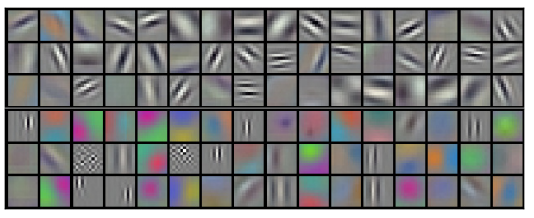
\includegraphics[width=.7\textwidth]{Images/cnnfilters.png}
    \caption{96 convolutionele filters\cite{Krizhevsky2012a}}
    \label{fig:cnnfilters}
\end{figure}

Daarna volgt een niet-lineaire laag. Deze kan een eenvoudige functie bevatten zoals een sigmo\"ide of de $\tanh$ functie, maar kan ook veel complexer zijn en bijvoorbeeld een ``rectified sigmoid'' bevatten, al dan niet gecombineerd met een normalisatie.

De laatste laag in elk niveau is een feature pooling laag die de dimensionaliteit van de output reduceert door regio's van de output te vervangen door hun gemiddelde of maximumwaarde. De maxima (of gemiddelde waarden) van alle regio's vormen dan een down-sampled weergave van de input. Figuur \ref{fig:maxpool} illustreert het principe van max-pooling met een filtergrootte van 2x2 en een stapgrootte van 2. 

\begin{figure}[tb]
    \centering
    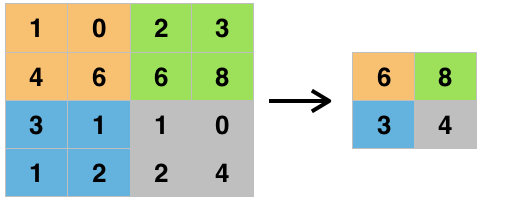
\includegraphics[width=0.6\linewidth]{Images/maxpool.png}
    \caption{Max pooling met 2x2 filter en stapgrootte 2}
    \label{fig:maxpool}
\end{figure}

De laatste fase in een traditionele convolutionele architectuur bestaat uit een aantal volledig verbonden lagen, gevolgd door een classificatielaag.

Trainen van dit netwerk kan gesuperviseerd met behulp van terugpropagatie, maar ook zeer snel ongesuperviseerd waardoor er geen nood is aan zeer grote gelabelde datasets. CNN's zijn in staat om veel sneller concepten te leren dan gewone feedforward netwerken, terwijl ze theoretisch slechts iets mindere resultaten kunnen bekomen. Een CNN gebruikt op elk niveau rechthoekige regio's uit de vorige laag die bovendien mogen overlappen. Door deze overlapping is het netwerk translatie-invariant.

E\'en van de meest succesvolle toepassingen van CNN's is objectdetectie. Deze vooruitgang was vooral te wijten aan een paper\cite{Krizhevsky2012a} die CNN's gebruikt voor het oplossen van de ImageNet challenge.\cite{Russakovsky2014}
Dit is een competitie waarin afbeeldingen moeten worden geclassificeerd in een aantal voorgedefini\"eerde categorie\"en. De gebruikte architectuur bestaat uit 8 lagen waarvan 5 convolutioneel en 3 volledig verbonden. Ze gebruiken bovendien verschillende technieken om overfitten te vermijden. Als classificatielaag gebruiken ze softmax zodat het netwerk een kansverdeling over de verschillende categori\"een leert. De architectuur kan worden gezien in figuur \ref{fig:AlexNet} en  is een variant op de standaardarchitectuur die hierboven werd beschreven. Dit netwerk was het best presterende netwerk voor de wedstrijd in 2012. Ondertussen zijn nog diepere architecturen voorgesteld die op dezelfde en recentere wedstrijden nog betere resultaten bekomen.

Het netwerk (VGGNet)\cite{Arge2015} dat wij gebruiken bestaat uit 16 lagen en is publiek beschikbaar met behulp van Caffe\cite{Jia2014}. De feature maps van verschillende outputlagen van dit netwerk dienen als input voor andere taken dan de ImageNet Challenge. Zo kan de output van de laatste laag voor de classificatielaag worden beschouwd als een representatievector voor de hele afbeelding. Output van de andere lagen is een representatie voor afbeeldingskenmerken op een niveau lager dan de volledige afbeelding.
\begin{figure}[tb]
	\centering
	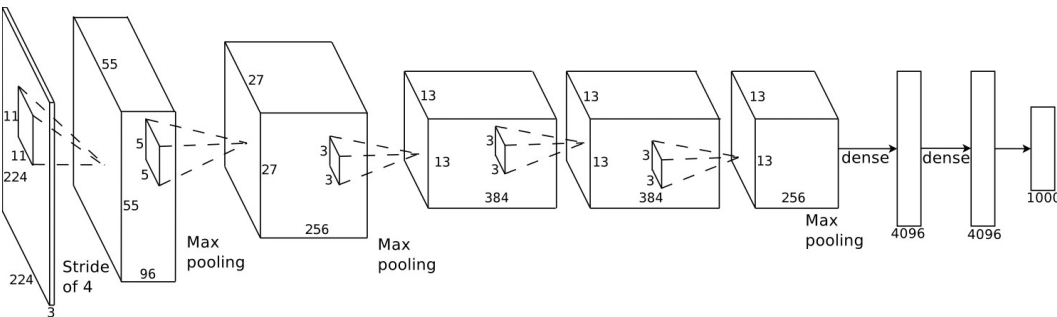
\includegraphics[width=\linewidth]{Images/cnn.PNG}
	\caption{Convolutioneel Neuraal Netwerk gebruikt door \cite{Krizhevsky2012a} voor classificatie van afbeeldingen}
	\label{fig:AlexNet}
\end{figure}

% RNN
\subsection{Recurrente Neurale Netwerken}
\todo[inline]{we hebben buiten word2vec geen enekele referentie in dit stuk?}
\todo[inline]{Referentie zoeken voor RNN}
Recurrente neurale netwerken zijn een uitbreiding van standaard feedforward neurale netwerken. Ze kunnen, net zoals feedforward netwerken, getraind worden met terugpropagatie. Het grote verschil met feedforward netwerken is de terugkoppeling van de output van de vorige stap naar de verborgen lagen. Op figuur \ref{fig:rnn} is een ontrolling van een RNN over verschillende tijdstippen te zien. $U,V$ en $W$ stellen gewichtsmatrices voor. Het ontrollen van het netwerk komt neer op het uitschrijven van het netwerk over verschillende tijdstippen. De pijlen van links naar rechts op de afbeelding komen overeen met de terugkoppeling van de output uit de vorige stap.

De terugkoppeling zorgt ervoor dat het netwerk in staat is om informatie te onthouden. Hierdoor kunnen recurrente netwerken tijdsgerelateerde informatie coderen. Daarom zijn ze geschikt om sequenti\"ele data, zoals tekst, te modelleren en te voorspellen. Recurrente neurale netwerken kunnen bijgevolg gebruikt worden als een taalmodel\cite{Mikolov2010}.

\begin{figure}[tb]
    \centering
    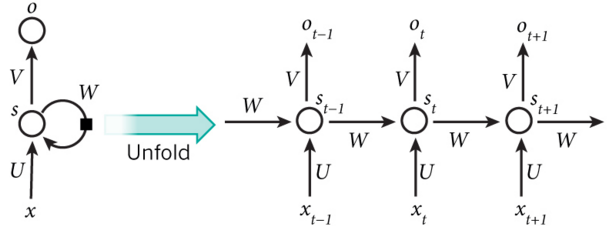
\includegraphics[width=\linewidth]{Images/rnn.PNG}
    \caption{Ontrolling van een recurrent neuraal netwerk\cite{RNNTutorial}}
    \label{fig:rnn}
\end{figure}

Het voorspellen van een zin met een RNN gebeurt woord per woord. Op basis van de eerder waargenomen woorden kan een softmax laag een kansverdeling maken voor het volgende woord. Met behulp van beam-search of het samplen van het meest waarschijnlijke woord, is het netwerk in staat om zinnen te genereren. Tijdens de trainingsfase worden woorden in de vorm van een vector aan het netwerk gegeven. Deze vectoren kunnen gebaseerd zijn op one-hot codering, ze kunnen random zijn, of het kunnen word embeddings zijn zoals bijvoorbeeld \texttt{word2vec}\cite{Mikolov2013}. Deze codering van woorden tot vectoren zelf kan ook deel uitmaken van het netwerk. Als dit het geval is, kan de codering verbeteren tijdens de training met behulp van terugpropagatie.

Een frequent probleem bij het trainen van dergelijke recurrente netwerken is de complexiteit van het netwerk. Hoe complexer het netwerk, hoe groter de kans op ``overfitting''. Hierbij is het uiteindelijke netwerk te hard afgestemd op de trainingsdata, waardoor de precisie op de testdata achteruit gaat. Om dit probleem aan te pakken biedt Srivastava\cite{Srivastava2013} een oplossing. Hij introduceert ``dropout'' om dit fenomeen tegen te gaan. Bij het gebruik van dropout laat het netwerk tijdens het trainen een aantal neuronen vallen. Bij elk trainingsvoorbeeld zijn er een aantal gewichten die waarde 0 krijgen, waardoor ze niet bijdragen aan de training. Een willekeurig proces bepaalt welke neuronen nul zijn in elke stap. Dit proces is aangestuurd door een parameter die de kans op dropout aangeeft per neuron. Deze  kans kan verschillend zijn voor elke laag: typisch is deze kans kleiner voor inputwaarden dan voor verborgen waarden.

Een tweede probleem is het gebrek aan aanpassing van de leersnelheid voor verschillende parameters. Hiervoor zijn een aantal oplossingen te vinden in de literatuur. Eern eerste is het gebruik van ``Adagrad''\cite{Duchi2011}. Hierbij maakt het algoritme gebruik van formule \eqref{formule:adagrad} om de gewichten aan te passen. Hierdoor zullen parameters waarbij de gradi\"ent zeer groot is een lagere effectieve leersnelheid hebben dan parameters met een kleinere gradi\"ent. In de formule staat $w$ voor de gewichtsvector, $dw$ is de grootte van de gradi\"ent, $\sigma$ is de learning rate, en $\epsilon$ is een smoothing parameter die deling door nul voorkomt. Een probleem dat kan voorkomen bij het gebruik van ``adagrad'' is dat het leerproces te vroeg stopt omdat de aanpassingen aan de leersnelheid te agressief zijn.
 
\begin{equation}
    w_t = w_{t-1} - \sigma \frac{dw}{\sqrt{dw^2} + \epsilon}
    \label{formule:adagrad}
\end{equation}

Soms biedt deze methode onvoldoende verbetering, bijvoorbeeld wanneer er negen voorbeelden zijn met gradi\"ent $0.1$ voor een bepaalde parameter, en het tiende voorbeeld heeft waarde $-0.9$. Dan kan ``rmsprop''\cite{RMSprop} een oplossing bieden. Deze techniek maakt gebruik van een bewegend gemiddelde over alle voorbije gradi\"enten om ervoor te zorgen dat grote schommelingen in de gradi\"ent slechts een kleine verandering in de gewichten aanbrengen. Formules \eqref{rmsprop:start}-\eqref{formule:rmsprop} toont hoe dit exact in zijn werk gaat. $\rho$ is de smoothing paramater voor het bewegende gemiddelde, $\sigma$ is de leersnelheid, $a_t$ is het gemiddelde op tijdstip $t$, $dw$ is de gradi\"ent en $w$ is de gewichtsvector. Ook hier vermijdt $\epsilon$ een mogelijke deling door nul.

\begin{eqnarray}
\vspace{-3mm}
    \label{rmsprop:start}
    a_t & = & \rho  a_{t-1} + (1 - \rho)dw^2 \\
    w_t & = &  - \sigma \frac{dw}{\sqrt{a_t} + \epsilon}
    \label{formule:rmsprop}
    \vspace{-3mm}
\end{eqnarray}

Een ander probleem met ``adagrad'' is dat de effectieve leersnelheid naar nul convergeert naarmate de training langer duurt. ``Adadelta''\cite{Zeiler2012} biedt hiervoor een oplossing door, net als rmsprop gebruik te maken van een bewegend gemiddelde, zowel voor gradi\"ent als voor gewichten. Door het gebruik van dit tweede gemiddelde is het niet nodig om expliciet een leersnelheid te defini\"eren. Formules \eqref{adadelta:start}-\eqref{formule:adadelta} tonen de exacte berekening van gewichtsupdates bij het gebruik van adadelta. $a_t$, $\rho$, $\epsilon$, $w$ en $dw$ zijn hetzelfde gedfini\"eerd als bij adagrad. $a_{wt}$ is het bewegende gemiddelde van de gewichten op tijdstip $t$ en $\Delta w_t$ is de aanpassing die gebeurt aan de gewichten op tijdstip $t$.

\begin{eqnarray}
\vspace{-3mm}
    \label{adadelta:start}
    a_t & = & \rho  a_{t-1} + (1 - \rho)dw^2 \\
    \Delta w_t & = & - \frac{\sqrt{a_{w(t-1)} + \epsilon}}{\sqrt{a_{t-1}}}dw \\
    a_{wt} & = & \rho  a_{w(t-1)} + (1 - \rho)\Delta w_t^2 \\
    w_t & = & w_{t-1} + \Delta w_t
    \label{formule:adadelta}
    \vspace{-3mm}
\end{eqnarray}


Twee andere vaak voorkomende problemen bij het trainen van recurrente neurale netwerken zijn exploderende en uitdovende gradi\"enten, waarbij de gradi\"ent van de fout tijdens de training enorm toeneemt, respectievelijk afneemt. Hiervoor zijn een aantal mogelijke oplossingen.

Een mogelijke oplossing is het gebruik van ``gradient clipping'' zoals voorgesteld door Pascanu et al.\cite{Pascanu2012}. Deze methode verkort de gradi\"entvector zodra de lengte van die vector boven een bepaalde drempel $t$ ligt en lost zo het probleem van exploderende gradi\"enten op. De update vindt dan plaats in de dezelfde richting, maar de norm is aangepast. Voor een vector $\mathbf{g}$ komt dit neer op volgende resulterende gradi\"entvector $\mathbf{\hat{g}}$:

\begin{equation}
    \mathbf{\hat{g}} = \frac{t}{||\mathbf{g}||}\mathbf{g}
\end{equation}

Het gebruik van Rectified Linear Units of ReLu-encodering biedt een oplossing voor het probleem van uitdovende gradi\"enten. Dit is een activatiefunctie die werkt volgens formule $ReLu(x) = max(x,0)$. Deze functie is zeer eenvoudig te berekenen en vermijdt uitdovende grade\"enten, in tegenstelling tot niet-lineaire functies zoals een sigmo\"ide of een hyperbolische tangens\cite{Glorot2011}.

Op lange termijn is het voor een RNN moeilijk om informatie te onthouden, net door deze exploderende en verdwijnende gradi\"enten. Hochreiter et al.\cite{SeppHochreiter1997} bieden met Long Short Term Memory netwerken een ander mogelijke oplossing voor dit probleem.

% LSTM
\subsection{Long Short Term Memory Neurale Netwerken}
\label{sub:lstm}
Long Short Term Memory (LSTM) is een vorm van RNN die geheugencellen bevat. Door deze cellen is het netwerk in staat om op lange termijn informatie over de input bij te houden. Elk LSTM blok heeft een aantal gates om te bepalen of de input moet onthouden worden, en of een vorige waarde moet bijgehouden of vergeten worden. De output van de cellen is bijgevolg afhankelijk van alle eerder geobserveerde inputs. Figuur \ref{fig:lstm} toont hoe een LSTM-blok er uitziet.\cite{SeppHochreiter1997,Google}

Op de figuur is duidelijk te zien hoe zowel input als output zijn teruggekoppeld naar de verschillende gates. De waarde van die gates hangt dus af van zowel de vorige voorspelling, als van de nieuwe input.

Formules \eqref{lstm-memory-start}-\eqref{lstm-memory} geven de exacte berekeningen weer die elke stap gebeuren. In deze formules zijn alle $W_{ij}$ gewichtsmatrices, $\sigma$ en $h$ zijn transferfuncties. $x$ is de input van het netwerk, $m_t$ is de output voor de softmaxlaag op tijdstip $t$ en $i'_t$, $f'_t$ en $o'_t$ zijn de waarden van respectievelijk input-, forget- en outputgate op tijdstip $t$. $c'_t$ is de waarde van de geheugencel op tijdstip $t$ en $p_t$ is de uiteindelijke voorspelling van het netwerk op tijdstip $t$. De $\odot$ operator stelt een puntsgewijze vermenigvuldiging tussen twee vectoren voor.

\todo[inline]{f veranderen in een o op tekening}

\begin{figure}[tb]
    \centering
    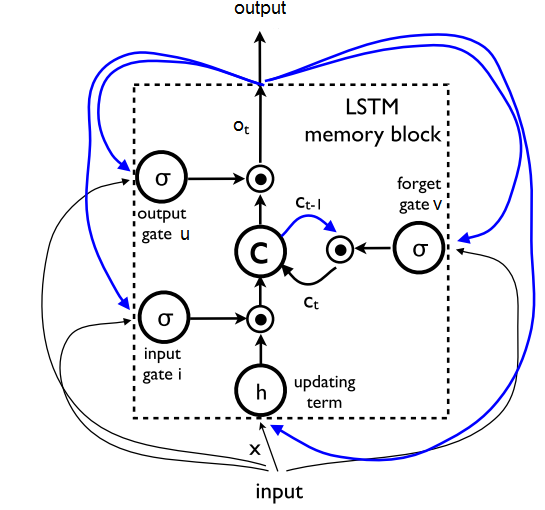
\includegraphics[width=\linewidth]{Images/lstm.PNG}
    \caption{Long Short Term Memory geheugenblok}
    \label{fig:lstm}
\end{figure}

\begin{eqnarray}
\vspace{-3mm}
\label{lstm-memory-start}
i_t' & = & \sigma (W_{ix} x_t + W_{im} m_{t-1}) \label{lstm-input} \\
f_t' & = & \sigma (W_{fx} x_t + W_{fm} m_{t-1}) \\
o_t' & = & \sigma (W_{ox} x_t + W_{om} m_{t-1}) \\
c_t' & = & f_t' \odot c_{t-1}' + i_t' \odot h(W_{cx} x_t + \nonumber \\
&   & + W_{cm} m_{t-1}) \\
m_t & = & o_t' \odot c_t'\\
p_{t+1} & = & SoftMax(m_t)
\label{lstm-memory}
\vspace{-3mm}
\end{eqnarray}

LSTM-netwerken worden net als RNN gebruikt als taalmodellen en zorgen over het algemeen voor hogere kwaliteit. Dit komt doordat LSTM-netwerken over een langere periode dan een gewoon RNN informatie kan onthouden. Dit maakt het modelleren van sequenties met events, die gescheiden zijn door een langere periode, mogelijk.


\section{Statistiek}

% LDA
\subsection{Latent Dirichlet Allocation}
Latent Dirichlet Allocation\cite{Blei2012} is een generatief probabilistisch model voor discrete data. E\'en van de meest gebruikte toepassingen hiervan is het modelleren van een een verdeling van onderwerpen in een set van tekstdocumenten. Dit concept veronderstelt dat elk document een zekere kansverdeling heeft over alle mogelijke onderwerpen. Deze onderwerpen hebben op hun beurt een kansverdeling over alle mogelijke woorden. Zo beschrijft formule \ref{formule:lda} de kans dat een bepaald document $d_j$ een bepaald woord $w_i$ bevat. 

\begin{equation}
    P(w_i | d_j) = \sum\limits_{k=0}^{n_{topics}}P(w_i|topic_k)P(topic_k|d_j)
    \label{formule:lda}
\end{equation}

Het generatieve aspect van LDA is te zien in algoritme \ref{algo:lda} en is ook ge\"illustreerd in figuur \ref{fig:lda}. Op basis van twee Dirichlet priors $\alpha$ en $\beta$ word een kansverdeling over de onderwerpen gesampled per document ($\theta$), alsook een kansverdeling over de woorden voor elk onderwerp ($\phi$). Deze priors geven de onzekerheid over de variabelen ($\theta$ en $\phi$) weer en dienen als basis voor een Dirichletverdeling\cite{Huang}. Een mogelijke interpretatie $\alpha$ is het aantal observaties van de verschillende topics alvorens het document in kwestie is gezien. Hetzelfde met $\beta$, dat het voorafgaand aantal samples van een bepaald woord uit een bepaald topic kan voorstellen. Uit $\theta$ wordt voor elke positie $i$ in een document $j$ een onderwerp gesampled ($z_{ji}$). Het samplen van de woordverdeling voor dit onderwerp leidt tot het woord $w_{ji}$\cite{LDAsien}.

\begin{algorithm}
\caption{Generatief aspect van LDA}
\begin{algorithmic} 
\STATE sample $K$ keer  $\phi \sim Dirichlet(\beta)$
\FORALL{document $d_j$}
\STATE sample $\theta \sim Dirichlet(\alpha)$
\FORALL{woord $i \in d_j$}
\STATE sample $z_ji \sim Multinomial(\theta)$
\STATE sample $w_ji \sim Multinomial(\phi,z_ji)$
\ENDFOR
\ENDFOR
\end{algorithmic}
\label{algo:lda}
\end{algorithm}

\begin{figure}[tb]
    \centering
    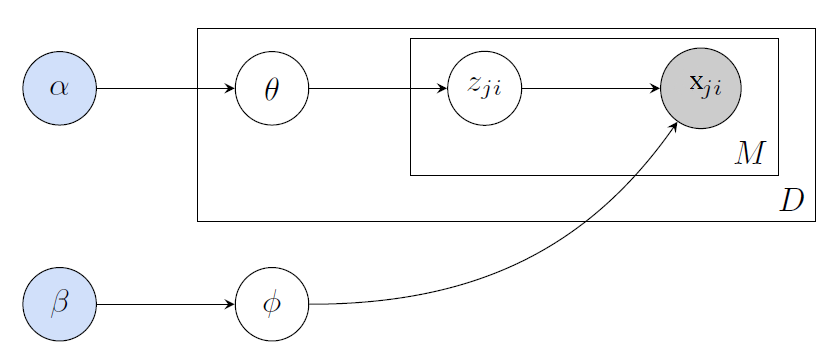
\includegraphics[width=\linewidth]{Images/lda.png}
    \caption{Grafische weergave van LDA}
    \label{fig:lda}
\end{figure}

Trainen van een LDA model gebeurt met een Markov chain Monte Carlo algoritme. Dit type algoritme construeert een Markovketen met als doel een kansdichtheidsfunctie te benaderen. De meest gebruikte techniek om een LDA model te benaderen is Gibbs sampling. Het uiteindelijke doel is het benaderen van de kansverdelingen $\theta$ en $\phi$.

Het trainen met Gibbs sampling begint met een random initialisatie van de topicverdeling voor elk document. Daarna itereert het algoritme over elk woord in elk document. Het berekent de kansverdeling over de verschillende topics, gebaseerd op de onderwerpen van de andere woorden in de collectie (update stap). De exacte berekening is terug te vinden in formule \eqref{lda:update}. Hierbij is $n_{j,k}$ het aantal toekenningen van onderwerp $k$ aan een woord in document $d_j$. $n_{j,k,\neg i}$ is het aantal keer dat topic $k$ is toegekend aan een woord in document $d_j$, woord $w_{ji}$ niet meegeteld. $n_{j,\cdot,\neg i}$ is de som van $n_{j,k,\neg i}$ over alle $K$ topics. $v_{k,w_{ji}}$ is het aantal associaties van woord $w_{ji}$ met topic $k$ in alle documenten, $v_{k,w_{ji}}$ is hetzelfde getal, maar dan zonder het huidige woord $w_ji$ mee te tellen. $v_{k,\cdot,\neg}$ is het totaal aantal woorden die bij topic $k$ horen, zonder $w_{ji}$ mee te tellen.

\begin{equation}
    P(z_{ji} = k | \mathbf{z}_{\neg ji}, \mathbf{w}, \alpha, \beta) \propto \frac{n_{j,k,\neg i} + \alpha}{n_{j, \cdot, \neg i} + K \alpha} \cdot \frac{v_{k,w_{ji}, \neg}+ \beta}{v_{k,\cdot,\neg} + |V|\beta}
    \label{lda:update}
\end{equation}

Op basis van deze kansverdeling wordt een nieuw topic gesampled voor het huidige woord, volgens formule \eqref{lda:sample}. Dit proces van updaten en samplen herhaalt zich tot er convergentie plaatsvindt. De geleerde topicverdelingen voor elk woord dienen dan als basis voor de topicverdelingen voor elk document en de woordverdelingen per topic. De berekening van de document-topicverdeling is te zien in formule \eqref{form:doctopic}, die voor topic-woordverdelingen in formule \eqref{form:topicword}. De symbolen hebben dezelfde betekenis als eerder beschreven.

\begin{equation}
    z_{ji} \sim  P(z_{ji} = k | \mathbf{z}_{\neg ji}, \mathbf{w}, \alpha, \beta)
    \label{lda:sample}
\end{equation}

\begin{equation}
    P(z_k|d_j) = \theta_{j,k} = \frac{n_{j,k} + \alpha}{\sum_{k^*=1}^K n_j,k^* + K\alpha}
    \label{form:doctopic}
\end{equation}

\begin{equation}
    P(w_i|z_k) = \phi_{k,i} = \frac{v_{k,w_i} + \beta}{\sum_{i^*=1}^{|V|} v_k,w_{i^*} + |V|\beta}
    \label{form:topicword}
\end{equation}


Het meest interessante voor deze masterproef zijn de topicverdelingen per document. Deze kunnen gebruikt worden als extra semantische informatie. De systemen kunnen op basis van dergelijke topicverdelingen een verband leren tussen de topics die voorkomen in de beschrijvingen, en de concepten die aanwezig zijn op de afbeelding. 



%  Stacked CCA
\subsection{Canonical Correlation Analysis}
\label{sub:stackedcca}
Canonical Correlation Analysis (CCA) is een methode die basisvectors probeert te vinden voor twee gerelateerde datasets. De bedoeling is om, bij projectie van overeenkomstige elementen uit beide datasets, een maximale lineaire correlatie te bekomen tussen de twee projecties. 
Op basis van singuliere waardenontbinding van de twee datasets is het mogelijk om deze ruimte te benaderen. Door het gebruik van singuliere waarden is het mogelijk om projecties in de tussenliggende ruimte te reduceren tot hun $n$ eerste componenten. Dit komt doordat een singuliere waarden ontbinding de dimensies van de basis gerangschikt zijn van dominant naar minder dominant. Voor een theoretische uitwerking en mogelijke oplossingsmethodes verwijzen we naar Weenink\cite{Weenink2003}.

In het onderzoek naar image captioning kan dit bijvoorbeeld leiden tot een multimodale mapping van afbeeldings- en beschrijvingsrepresentatie.

\paragraph{Stacked CCA}

Stacked Auxiliary Embedding\cite{Gong2014} kan op basis van extra informatie een verbeterde mapping maken. Een voorbeeld hiervan is een dataset van geannoteerde foto's, versterkt met per foto een set van stukjes van de foto met een bijbehorende beschrijving. De representaties van de foto's en annotaties uit de dataset kunnen verbeterd worden door gebruik te maken van de informatie uit de extra dataset.

Om de uiteindelijke augmentatie te bereiken, zijn er een aantal stappen nodig. Uit de extra dataset volgt een eerste set van CCA projecties ($A$, $B$). Daarna volgt een projectie van de originele dataset ($X$, $Y$) naar de multimodale ruimte, door vermenigvuldiging met $A$ en $B$, resulterend in projecties $AX$ en $BY$. Vervolgens transformeren we $AX$ en $BY$ volgens de niet-lineaire functie $\phi(x)$, zoals voorgesteld in de originele paper.

Concatenatie van de originele dataset met het resultaat van de niet-lineaire transformatie leidt tot $\hat{X} = [X, \phi(XA)], \hat{Y} = [Y, \phi(YB)]$. Een laatste stap in het proces is het berekenen van een CCA projectie die gebaseerd is op $\hat{X}$ en $\hat{Y}$, wat resulteert in $U$ en $V$.

Om de dimensionaliteit van de projectie te verhogen wordt voor $\phi(x)$ een random Fourier Feature (RFF) mapping gebruikt. Deze RFF is een functie gebaseerd op de gemiddelde afstand tot de vijftigste dichtste buur van de inputvector. Voor elke foto en caption wordt gekeken welke andere foto of caption de vijftigste dichtste buur is, om vervolgens het gemiddelde te nemen van alle afstanden. De exacte berekening is $\phi(\mathbf{x})=\sqrt{2}cos(\mathbf{x}R+\mathbf{b})$. Hierin is $R$ een matrix die verkregen wordt door sampling van een normaalverdeling met gemiddelde 0, en standaardafwijking $\sigma^2$, waarbij $\sigma$ overeen komt met de eerder berekende gemiddelde afstand. Vector $b$ is resultaat van sampling uit een uniforme verdeling [0,1].

De projectie van een ongeziene afbeelding is het resultaat van het achtereenvolgens uitvoeren van alle transformaties. Voor vector $\mathbf{x}$ geeft dit $\mathbf{\hat{x}} = U[\mathbf{x}, \phi(A\mathbf{x})]$. Deze representatie kan gebruikt worden als een verbeterde versie van de originele image vector, bijvoorbeeld bij een image retrieval taak.

\chapter{Methodologie}
Dit hoofdstuk beschrijft het proces van de implementatie van ons systeem. Een eerste sectie handelt over een bestaande implementatie, waarop ons systeem is gebaseerd. Een tweede sectie beschrijft onze eigen extensie van de code van Karpathy, meer specifiek hoe we LDA topic verdelingen gebruiken om extra semantische informatie toe te voegen. Een derde sectie gaat over onze implementatie van het eerder vernoemde gLSTM netwerk zoals voorgesteld door Jia \todo{reference?}. De laatste sectie beschrijft hoe wij een normalisatie hebben toegevoegd aan de beam search om zinnen te maken (zoals voorgesteld door Jia \todo{ref}).

\section{Startpunt Karpathy} \todo{Betere titel}
Het startpunt van onze implementatie is de code aangereikt door A. Karpathy op zijn github pagina. Die bevat een implementatie van het recurrente neurale netwerk beschreven in \todo{reference naar karpathy}, alsook een implementatie die gebaseerd is op \todo{reference vinyals}. Op basis hiervan hebben wij een aantal extensies ge\"implementeerd.
\subsection{Recurrent Neuraal Netwerk}
Een eerste implementatie waarvan we zijn vertrokken is beschreven in Karpathy\todo{ref!}. Hij beschrijft een systeem dat op basis van een afbeelding een beschrijvende zin genereert. Dit gebeurt in twee stappen. Eerst wordt de afbeelding door middel van een CNN omgezet naar een vector representatie. Deze vector dient vervolgens als input voor een recurrent neuraal netwerk.

\paragraph{Afbeeldingsrepresentatie}

\paragraph{Van afbeelding naar beschrijving}
De berekende vector representatie van de afbeelding dient als input voor een recurrent neuraal netwerk. Tijdens de training van het netwerk wordt op basis van de afbeelding, in combinatie met een speciale startvector die het begin van een zin aangeeft, het eerste woord voorspeld. Daarna wordt op basis van het eerste woord van de zin een voorspelling gemaakt voor het tweede woord. Dit proces herhaalt zich tot het einde van de zin bereikt is. Terugpropagatie op basis van stochastic gradient descent zorgt voor de juiste wijzigingen aan de gewichten van het netwerk. Een eenvoudige weergave dit proces is te zien op figuur \ref{fig:rnntraining}.

\begin{figure}[tb]
    \centering
    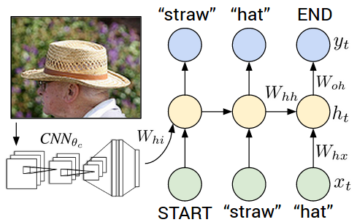
\includegraphics[width=0.5\linewidth]{Images/karpathy.PNG}
    \caption{Generatie van caption met recurrent neuraal netwerk}
    \label{fig:rnntraining}
\end{figure}

Het genereren van captions gebeurt op basis van beam search. Hierbij wordt op basis van de afbeelding een ranking gemaakt van de meest waarschijnlijke eerste woorden voor de zin. De eerste $n$ woorden dienen dan als startpunt van de voorspelling van het tweede woord. Over alle mogelijke sets van twee woorden wordt opnieuw een rangschikking gemaakt, waarvan de $n$ beste resultaten worden bijgehouden. Dit proces herhaalt zich tot elke vertakking van de zoekboom is onderzocht, waarna de beste gegenereerde zin wordt gebruikt als eindresultaat.


\subsection{Long Short Term Memory Netwerk}

\section{Toevoeging van LDA topicverdeling aan RNN}


\section{gLSTM}



\section{Normalizatie van beam search}
\chapter{Evaluatie}
\label{hoofdstuk:evaluatie}
Dit hoofdstuk behandelt enkele gebruikte methodes om de ontwikkelde systemen te evalueren. Twee van deze methodes vinden hun oorsprong in de computervertaling. Ze zijn ontwikkeld om automatisch de kwaliteit van vertalingen te meten. Het doel van deze evaluatiealgoritmes is om zo goed als mogelijk menselijke evaluatiescores te benaderen. De laatste vorm van evaluatie kijkt naar statistieken van de gegenereerde zinnen.


\section{Automatische evaluatie}
Om verschillende systemen te kunnen vergelijken, moet er een manier zijn om de gegenereerde zinnen te evalueren. Elke zin moet aan twee belangrijke voorwaarden voldoen. Enerzijds moet de inhoud van de zin overeenkomen met de inhoud van de afbeelding. Anderzijds moet de zin een grammaticaal correcte structuur hebben en voldoende vloeiend zijn.

Ideaal gezien beoordelen meerdere mensen elke zin om tot een betrouwbare evaluatie van beide eigenschappen te komen. Deze beoordeling kan bijvoorbeeld door een score te geven op de kwaliteit van elke zin. Een andere optie is om proefpersonen te laten oordelen of een automatisch gegenereerde zin beter, gelijkaardig of slechter is dan de overeenkomstige referentiezin. Het nadeel van elk van deze methodes is de nood aan meerdere proefpersonen die voor elke gebruikte methode of instelling van de netwerken, alle duizend zinnen van de validatieverzameling of de testverzameling moet beoordelen. Het is duidelijk dat dit een kostelijke operatie is. Daarvoor bieden automatische evaluatiealgoritmes een oplossing. Het nadeel van deze methodes is dat ze niet perfect overeenkomen met de menselijke evaluatie.

In wat volgt bespreken we eerst twee algoritmes uit de computervertaling, namelijk BLEU\cite{Papineni2001} en Meteor\cite{Denkowski2007a}. Deze algoritmes zijn bruikbaar omdat de gegenereerde zinnen kunnen worden beschouwd als ``vertalingen'' van de afbeeldingen. Het is aangetoond dat de twee methodes correleren met menselijke evaluaties van gegenereerde zinnen. Van de gebruikte methodes heeft Meteor de hoogste correlatie\cite{Elliott2014}.
Geen van beide algoritmes is echter perfect voor het meten van de kwaliteit.
Om die reden bekijken we ook nog enkele statistieken van de gegenereerde zinnen om hieruit andere interessante fenomenen af te leiden.
Als laatste onderdeel volgt een bespreking van een methode die de laatste twee jaar in onbruik is geraakt binnen dit onderzoeksdomein. Deze methode is gebaseerd op een rangschikking van zinnen en afbeeldingen. Deze rangschikking leidt tot een numerieke score voor de bekomen resultaten.

\section{BLEU}
Kort gesteld berekent het BLEU-algoritme scores van computervertalingen op basis van overeenkomsten met de referentiezinnen. Deze overeenkomsten bestaan uit gemeenschappelijke woorden of opeenvolgingen van gemeenschappelijke woorden. Verschillende vormen van BLEU kunnen worden gebruikt afhankelijk van het aantal gebruikte woorden in een opeenvolging (n-grams) \todo{deze zin is vaag, ma ik weet ni wa ge bedoelt dus ik kan het ni verbeteren -> beter?}. Het gebruik van BLEU heeft echter wel enkele nadelen.

\subsection{Algoritme}
Om de n-gram BLEU-score van een zin te berekenen bepaalt het algoritme eerst de \textit{modified n-gram precision} of gewijzigde n-gram precisie. Dit is een vorm van precisie die rekening houdt met het aantal keer dat elk woord in de referentiezinnen voorkomt. Op deze manier krijgen zinnen als \texttt{the the the the the} een lage score omdat \texttt{the} nooit vijfmaal voorkomt in een referentiezin. 

De berekening van de gewijzigde n-gram precisie gebeurt door eerst het maximum te nemen van het aantal keer dat een specifieke woordsequentie voorkomt in elke referentiezin. Vervolgens telt het algoritme het aantal voorkomens ($Count(ngram)$) van deze sequentie in de gegenereerde zin $s$. Het minimum van deze twee getallen ($Count_ {clip}$) wordt dan voor elk woord in de vertaalde zin opgeteld en gedeeld door het totaal aantal woorden in de gegenereerde zin.

\begin{equation}
p_{modified}(s) =
\frac{\sum\limits_{ngram \in s} Count_{clip}(ngram)}{\sum\limits_{ngram' \in s} Count(ngram')}
\label{formule:ngramprecision}
\end{equation}
Vanuit deze formule volgt een score voor een volledige corpus van gegenereerde zinnen als volgt:
\begin{equation}
p_{n} =
\frac{\sum\limits_{C \in \{Candidates\} } \sum\limits_{ngram \in C} Count_{clip}(ngram)}{\sum\limits_{C' \in \{Candidates\} } \sum\limits_{ngram' \in C'} Count(ngram')}
\label{formule:corpus_modified}
\end{equation}
Hierin is $Candidates$ de verzameling van alle gegenereerde zinnen.

Vanuit deze scores voor $n=1$ tot en met $N$ is het mogelijk om een N-gram BLEU-score te bepalen. Dit gebeurt door het gemiddelde logaritme te nemen met uniforme gewichten $w_n$, wat overeenkomt met het geometrisch gemiddelde van de gewijzigde n-gram precisies.
\begin{equation}
BLEU = exp(\sum\limits_{n=1}^N w_nlog(p_n))
\end{equation}
Deze score dwingt echter niet de juiste lengte van de zin af. Om die reden bepaalt Papineni een extra multiplicatieve factor, namelijk de Brevity Penalty ($BP$). Voor elke gegenereerde zin bepaalt het algoritme de referentiezin met de dichtstbijzijnde lengte. De lengte daarvan noemt de paper de ``beste match lengte''. Vervolgens worden zowel de lengtes van de gegenereerde zinnen als de beste match lengte opgeteld tot respectievelijk $c$ en $r$. Berekenen van de Brevity Penalty kan dan met volgende formule:
\begin{equation}BP=
 \begin{cases}
1 & if c > r \\
e^{1-r/c} & else
\end{cases}
\end{equation}

De uiteindelijke BLEU-N score is dan gelijk aan:
\begin{equation}
BLEU = BP\cdot exp(\sum\limits_{n=1}^N w_nlog(p_n))
\end{equation}
Hierbij is $w_n$ gelijk aan $1/N$ wanneer het uniforme geometrisch gemiddelde wordt genomen.

\subsection{Nadelen en gebruik}
De BLEU-score is de meest gebruikte gebruikte evaluatiemethode in de literatuur. De meeste papers die afbeeldingsbeschrijvingen genereren bespreken BLEU-1 tot BLEU-4 scores. De literatuur lijkt het echter niet eens over het gebruik van de Brevity Penalty. Sommige papers vermelden expliciet dat ze het niet gebruiken, maar andere volgen de paper van Papinemi volledig. Door dit verschil in evaluatie is de vergelijking van verschillende systemen niet altijd eerlijk. Wanneer de gegenereerde zinnen lang genoeg zijn komen de scores wel overeen.
In onze experimenten stellen we de Brevity Penalty steeds gelijk aan 1.

Naast deze problemen zijn er verschillende implementaties met kleine onderlinge verschillen. De meeste van deze verschillen vinden in hun oorsprong in het al dan niet toevoegen van normalisatie. Hierdoor zijn de concrete scores dus afhankelijk van de gebruikte implementatie. In onze experimenten gebruiken we de \texttt{multi-BLEU.pl}\footnote{\url{https://github.com/moses-smt/mosesdecoder/blob/master/scripts/generic/multi-bleu.perl}} code uit de Moses decoder\cite{Koehn2006} omdat Karpathy deze ook voorziet in zijn code.

Elliot et al.\cite{Elliott2014} tonen aan dat BLEU slechts een matige correlatie heeft met menselijke beoordeling.
Hiervoor zijn meerdere verklaringen mogelijk. Zo kijkt BLEU enkel naar exacte woordmatches maar houdt het geen rekening mee met semantisch gelijkaardige woorden. Het gebruik van een synoniem in plaats van hetzelfde woord bijvoorbeeld geeft geen hogere score, terwijl dit bij menselijke evaluaties wel zo is. Daarnaast krijgen woorden die weinig semantische waarde bevatten een evengrote score als woorden die veel meer informatie over de afbeelding geven. Concreet geeft dus een woord als \texttt{a} evenveel extra score als een woord als \texttt{ski}. Ook werkwoorden die semantische informatie bevatten die in de referentiezin als substantief voorkomen geven problemen. Hieronder volgen voorbeelden van situaties waarbij zinnen slecht scoren volgens BLEU, maar inhoudelijk toch hetzelfde weergeven.
\\

Reference 1: \texttt{Two boys are on their bikes.}

Candiate 1: \texttt{Two boys are on their bicycles.}

Reference 2: \texttt{A man is skiing down a hill.}

Candidate 2: \texttt{A man is going down a hill on his skis}
\\

Meteor is een evaluatiealgoritme met als doel het vermijden van dergelijke foute evaluaties.

\section{Meteor}
Elliott et al.\cite{Elliott2014} tonen aan dat zeker unigram BLEU (B1) slechts een zwakke correlatie heeft met menselijke evaluatie. Hogere orde BLEU-scores hebben slechts een matige correlatie. Meteor is een metriek die specifiek ontworpen is om de tekortkomingen van BLEU te verbeteren. Van de door Elliott onderzochte evaluatiemechanismen, correleert Meteor het beste met menselijke evaluatie.

\subsection{Algoritme}
Meteor\cite{Denkowski2007a} evalueert vertaalde zinnen door ze te aligneren met de referenties en hiervan per zin een score te berekenen. Bij het berekenen van de score wordt net zoals bij BLEU gekeken naar de precisie. Daarnaast heeft in contrast met BLEU ook de recall een invloed. De paper bevat een implementatie in de vorm van een JAR-bestand, zodat er geen twijfel bestaat over het gebruik van het algoritme.

Concreet probeert het algoritme twee zinnen te aligneren met behulp van vier matchers. Als eerste is er een match wanneer de woordvormen exact dezelfde zijn. Als tweede is er een match wanneer met een Snowball Stemmer\cite{porter2001snowball} ``gestemde'' woorden gelijk zijn. Een derde matcher kijkt naar overeenkomsten in de WordNet synoniemenlijst van elk woord\cite{Miller1990}. Als laatste vormen frases of woordsequenties een match wanneer ze in zogenoemde parafrasetabellen voorkomen. Een parafrasetabel bevat paren tussen frases en parafrases die ermee overeenkomen. Parafrases zijn woordsequenties die dezelfde betekenis hebben dan de overeenkomstige frase, maar op een andere manier geformuleerd zijn.
Elke matcher heeft een bepaald gewicht. De experimenten gebruiken de standaardgewichten 0.85, 0.2 ,0.6 en 0.75.

Uiteindelijk worden alle matches gegeneraliseerd tot frase matches met een bepaalde startpositie en eindlengte. Een van de doelen van de Meteor score is om zoveel mogelijk woorden af te dekken in de twee zinnen. Daarnaast moet het aantal \textit{chunks} minimaal zijn. Denkowski et al. defini\"eren een chunk als aaneengesloten en identiek geordende matches tussen de twee zinnen. De uiteindelijke Meteor score bestaat dan uit de F-score $F_{mean}$ vermenigvuldigd met een penalisatiefactor $Pen$ op basis van het aantal chunks.


\begin{equation}
Score = (1 - Pen)*F_{mean}
\end{equation} 
\begin{equation}
Pen = \gamma (\frac{ch}{m})^\beta 
\end{equation}
\begin{equation}
F_{mean} = \frac{PR}{\alpha P + (1- \alpha)R}
\end{equation}
Hierbij zijn $P$ en $R$ respectievelijk de gewogen precisie en recall van de gealigneerde unigrams ($m$) tussen kandidaat- en referentiezin. $m$ is het gemiddeld aantal gematchte woorden. $ch$ is het aantal chunks. $\alpha$,$\beta$ en $\gamma$ zijn vooraf getrainde parameters.

Wanneer er meerdere referenties zijn in het corpus, bepaalt het maximum van de individuele scores voor elke referentie de score van de vertaling.

\subsection{Gebruik en nadelen}
Zoals al aangehaald toonden Elliott en Keller in 2014 aan dat van de bestudeerde evaluatiemethodes Meteor de hoogste correlatie heeft met menselijke beoordelingen voor afbeeldingsbeschrijvingen. Om deze reden rapporteren wij ook de resultaten met dit algoritme. In de literatuur blijven BLEU-scores echter de meest gerapporteerde resultaten.

Ondanks dat het het meest performante algoritme is, vertoont Meteor nog steeds slechts matige correlatie met menselijke beoordelingen. Verder onderzoek naar betere automatische evaluatie kan dus nuttig zijn. Daarnaast vereist het tabellen en synoniemenlijsten die niet voor elke taal beschikbaar zijn. Voor het Engels is deze informatie echter wel beschikbaar. 


\section{Extra informatie uit de gegenereerde zinnen}
Naast de automatische algoritmes die aan elk model een duidelijke score geven, bevatten de gegenereerde zinnen van bijvoorbeeld de validatieverzameling nog andere interessante statistieken. Deze statistieken hebben niet altijd een rechtstreeks verband met de kwaliteit van de zinnen. Ze geven wel informatie die nuttig kan zijn om het gebruikte model te analyseren en te verbeteren.

Een eerste vorm van informatie ligt in de verdeling van de lengtes van de zinnen. Ons systeem biedt de mogelijkheid om voor elke aanwezige lengte in de bestudeerde verzameling het aantal zinnen te bepalen. Hierdoor is het onder andere mogelijk om uitschieters vast te stellen. Ook maakt het de detectie van vermoedelijk foutieve zinsconstructies mogelijk. Het aantal zinnen van lengte twee, drie of bijvoorbeeld meer dan twintig geeft een goede indicatie van de neiging om inhoudsloze zinnen te genereren. Daarnaast berekent het systeem ook de gemiddelde lengte en vergelijkt het deze met de gemiddelde lengte van de referentiezinnen. Dit maakt duidelijk of het model een voorkeur heeft voor bijvoorbeeld korte zinnen.

De gebruikte woordenschat en bijbehorende woordfrequenties bieden een tweede bron van informatie. Het aantal unieke woorden geeft een idee van hoe gevarieerd het woordgebruik is van het model. Als dit aantal aan de lage kant is, is de kans groter dat het model veel dezelfde uitdrukkingen en bij uitbreiding zinnen genereert. Daarnaast evalueren we ook het aantal voorkomens van de gebruikte woorden. Dit geeft dus informatie over de voorkeur voor bepaalde woorden. De vergelijking van deze voorkeur met deze van de referentiezinnen kan dan leiden tot het ontdekken van bepaalde eigenschappen van het model.

Een derde optie bestaat erin om te kijken hoeveel unieke zinnen het systeem genereert. Onze implementatie biedt de mogelijkheid om de gegenereerde zinnen voor de testverzameling te vergelijken met die in de trainingsverzameling. Dit geeft een beeld van in welke mate het model echt nieuwe zinnen genereert of gekende zinnen teruggeeft. Daarnaast is er de mogelijkheid om het aantal echt unieke zinnen te berekenen. Dit zijn zinnen die niet in de trainingsverzameling voorkomen of al gegenereerd zijn. Zo is het mogelijk om een beeld te vormen van hoe gevarieerd het systeem is in het genereren van zinnen. 

\section{Afbeelding-zin rangschikking}
Enkele oudere werken in de literatuur over automatische afbeeldingsbeschrijving gebruiken nog een andere vorm van evaluatie. Hodosh introduceerde deze vorm van evolueren voor dit type van problemen\cite{Hodosh2013}. Hij defini\"eert twee types van evaluatie op basis van het opzoeken van een gezochte zin of afbeelding. Enerzijds met als startpunt een afbeelding, waarbij beschrijvende zinnen worden gezocht (sentence retrieval). Anderzijds zoekt men afbeeldingen op basis van een zin (image retrieval). Voor foto's bijvoorbeeld moet een systeem dan een rangschikking van de zinnen bij elke foto produceren. Vervolgens vormt de positie $r$ van de eerste correcte zin de basis van de score. De eenvoudige maar veelgebruikte metriek $recall @ k$ wordt gebruikt voor evaluatie. Hierbij vormt het percentage van de afbeeldingen waarbij de correcte zin bij de eerste $k$ zinnen zit de uiteindelijke score. Ook de mediaan van de gevonden posities ($med\: r$)wordt dikwijls vermeld. Hetzelfde principe werkt ook in de omgekeerde richting. Hierbij gaat men van een zin via het model terug naar een rangschikking van afbeeldingen. Deze laatste manier van evalueren toont aan hoe het gebruikte model kan worden gebruikt om gekende afbeeldingen te zoeken op basis van nieuwe queries. 

Volgens Vinyals et al.\cite{Google} is de transformatie van generatie naar rangschikking echter geen gerechtvaardigde evaluatiemethode. Naarmate afbeeldingen en daarbij ook het woordenboek complexer worden, groeit het aantal mogelijke zinnen exponentieel. Hierdoor daalt de likelihood van de voorgedefin\"ieerde zinnen, tenzij het aantal van deze zinnen ook exponentieel stijgt. Dit is geen realistische veronderstelling en maakt de evaluatie computationeel onhaalbaar. Omwille van deze redenering verdwijnt $recall @ k$ in de meer recente papers en gebruiken wij deze evaluatiemethode ook niet. Tabel \ref{table:recall} geeft een voorbeeld van de afbeelding-zin rangschikking in beide richtingen. Dit zijn de resultaten zoals weergegeven in de paper van Vinyals. Opvallend is hier dat de gevonden scores zeker niet veel beter zijn dan de referentiescores, terwijl zijn model wel veel beter scoort op de automatische evaluatiemethodes (BLEU-N). Van deze laatste methodes is bovendien de correlatie met menselijke evaluatie wel aangetoond.


\begin{table}
	\centering
	\begin{small}
		\setlength{\tabcolsep}{3pt}
		\begin{tabular}{|c|ccc|ccc|}
			\hline
			\multirow{2}{*}{Approach} & \multicolumn{3}{c|}{Image Annotation} & \multicolumn{3}{c|}{Image Search} \\
			& R@1 & R@10 & Med $r$ &  R@1 & R@10 & Med $r$ \\
			\hline
			\hline
			DeFrag~\cite{Karpathy2014} & 16 & 55 & 8             &    10 & 45 & 13  \\
			m-RNN~\cite{Mao2014}         &  18 & 51 & 10               &  13 & 42 & 16\\
			MNLM~\cite{Kiros2014}        &  \textbf{23}   & \textbf{63} & \textbf{5}        &  \textbf{17} & \textbf{57} & \textbf{8}   \\
			\hline
			NIC~\cite{Google}                           &  17 & 56  & 7               &    \textbf{17} & \textbf{57} & \textbf{7} \\
			\hline
		\end{tabular}
	\end{small}
	\caption{Recall@k and mediaan van de rang op Flickr30k uit de NIC paper.\label{tab:recall@1030k}}
	\label{table:recall}
\end{table}




%%% Local Variables:
%%% mode: latex
%%% TeX-master: "masterproef"
%%% End:

\chapter{Experimenten} % (fold)
\label{cha:experimenten}
Dit hoofdstuk bevat een overzicht van de experimenten die zijn uitgevoerd. Enerzijds zijn er experimenten die de modellen trainen en evalueren om absoluut betere resultaten te halen dan het basismodel. Anderzijds bekijken we het effect van ruis op twee gLSTM implementaties.

\section{Eigen implementaties} % (fold)
\label{sec:eigen_implementaties_exp}
Het doel van deze masterproef is om de basisresultaten van de paper en bijbehorende implementatie van Karpathy\cite{Karpathy2015} te verbeteren. Om die reden volgen we nauwgezet dezelfde types van experimenten. Daarom doet hetzelfde VGGNet met 16 lagen dienst als convolutioneel netwerk. Daarnaast voeren we alle experimenten uit op de Flickr30k dataset en gebruiken we dezelfde test-, train- en validatiedeelverzameling als deze in de paper. We trainen het netwerk en de toegevoegde uitbreidingen met behulp van de trainingset. Het afstellen van de parameters van deze modellen gebeurt op basis van scores op de validatieset. De uiteindelijke evaluatie gebeurt op de testset. Op deze manier is geen enkel model getraind op de test set en kan een correcte vergelijking gebeuren met de rest van de literatuur.

We vermoeden echter dat Karpathy gebruik maakt van een brevity penalty \todo{quotes?} bij de Bleu scores. In dit werk en in andere werken in de literatuur gebeurt dit echter niet. Om die reden doen we eerst experimenten met de standaard instellingen van de code van Karpathy voor zowel het RNN als LSTM model. De resultaten hiervan vormen dan de referentiewaarden die moeten worden verbeterd. 

De verschillende modellen zijn getraind met de volgende instellingen: leersnelheid 0.0001, type solver rmsprop, decay rate 0.999, epsilon smoothing 1e-8, batch-size 100, gradient clipping 5, dropout in encoder en decoder 0.5. \todo{Dit fixen :D}

Beam search is het algoritme dat zorgt voor het genereren van de zinnen. In onze experimenten is de beam-grootte steeds 50.
BLEU-scores (1-4), METEOR-scores en enkele statistieken dienen als evaluatiemetriek. Deze scores zijn berekend met behulp van steeds vijf referentiezinnen.

Naast de referentiewaarden voeren we ook experimenten uit op onze eigen geschreven uitbreidingen.
Deze bevatten RNN uitgebreid met LDA, gLSTM met CCA voor verschillende groottes van CCA-vector, gLSTM met LDA voor verschillende groottes van topics. Daarnaast bekijken we ook het effect van Gaussiaanse normalisatie en Min-Hinge normalisatie op elk van deze modellen.

\section{Ruisgevoeligheid van CCA en LDA} % (fold)
\label{sec:ruisgevoeligheid_van_cca_en_lda_exp}
gLSTMS maken het mogelijk om extra semantische informatie aan het taalmodel te geven. Deze informatie kan uit verschillende bronnen komen. In deze masterproef bekeken we CCA en LDA. Naast de absolute scores van de twee modellen is het ook interessant om te kijken naar de robuustheid tegen ruis in de referentiezinnen.
Om deze eigenschap te evalueren cre\"eren we een nieuwe dataset waarbij de referentiezinnen van de trainingsset perturbaties bevatten.
Concreet wordt elk woord vervangen door een willekeurig woord in het vocabularium met een kans van 10\%. Hierna traint het netwerk op dezelfde manier als hierboven beschreven. Na deze training en generatie van resultaten op de testverzameling is het mogelijk om te vergelijken welk model relatief het meeste last heeft van deze extra ruis in de dataset.

% section besluit (end)


\chapter{Resultaten} % (fold)
\label{cha:resultaten}
Dit hoofdstuk bevat de resultaten van de verschillende experimenten die zijn uitgevoerd. Eerst bespreken we de resultaten van de verschillende uitbreidingen met hun overeenkomstige referentiemodel. Daarna volgt een beschouwing van de invloed van verschillende parameters op de resultaten. Dan volgt een kritische vergelijking van de beste modellen met de state-of-the art resultaten. Een laatste set van experimenten gaat over een vergelijking van CCA en LDA als gids voor de gLSTM implementatie. Meer specifiek focust  de vergelijking op hoe deze twee presteren bij aanwezigheid van ruis in de trainingsdata.

\section{Vergelijking eigen toevoegingen met referenties}  % (fold)
\label{sec:eigen_implementaties}
Zoals vermeld in het vorige hoofdstuk defini\"eren we een referentiemodel getraind met de basisinstellingen voor zowel RNN als LSTM. Deze sectie bespreekt het effect van het toevoegen van LDA aan het RNN-netwerk, het effect van de twee gidsen op het LSTM-netwerk en het effect van normalisatie bij de beam-search op beide netwerken. Er volgt steeds eerst een bespreking van de automatische evaluatie gevolgd door een analyse van de verzamelde statistieken van elk model.

\subsection{RNN}
Zoals al vermeld evalueert Karpathy~\cite{Karpathy2015} de Bleu-score met een Brevity Penalty. Hij voorziet ook geen informatie over Meteor of andere statistieken. Daarom voeren we eerst experimenten uit met de basisinstellingen voor RNN (\emph{ref-RNN}) zonder Brevity Penalty. Hierbij wordt op elk tijdstip de afbeelding aan het netwerk meegegeven. De resultaten van Karpathy krijgen niet op elke tijdstap de afbeelding mee. Hij rapporteert dat dit nog beter presteert. Wanneer de evaluatie toch met Brevity Penalty gebeurt, toont tabel~\ref{table:karpathy_met_bp} dat de referentie toch zeer sterk overeenkomt met de resultaten van de paper van Karpathy. 

\begin{table}
	\begin{tabular}{lllllll}
		& Bleu-1 & Bleu-2 & Bleu-3 & Bleu-4 & Meteor \\ \hline
		RNN (Karpathy~\cite{Karpathy2015})    & 57.3   & 36.9   & 24     & 15.7   & ~           \\    
		ref-RNN + BP     & 55.17   & 36.64   & 23.89   & 15.13   & 14.29          \\
		ref-RNN          & 64.9  & 43.1     & 28.1   & 17.8   & 14.29          \\
	\end{tabular}

	\caption{Resultaten Karpathy~\cite{Karpathy2015} in vergelijking met onze referentieresultaten.}
	\label{table:karpathy_met_bp}
\end{table}

Tabel~\ref{table:rnn_met_lda} toont het effect van het toevoegen van LDA aan de basisimplementatie van RNN. Alle gebruikte metrieken vertonen een stijging. LDA lijkt er dus in te slagen om de semantische drift tegen te gaan.
Het toevoegen van Gauss-normalisatie verbetert steeds de score van Bleu-4 en Meteor. Dit zijn de scores die het meest overeenkomen met menselijke evaluatie. Net zoals Jia et al.~\cite{Fernando2015} al aanhaalden lijkt de bias van standaard beam-search lagere Bleu-scores te bevoordelen. Zo domineren de korte zinnen dus niet enkel de gegenereerde zinnen, maar be\"invloeden ze ook de evaluatie.

\begin{table}
	\begin{tabular}{lllllll}
		& Bleu-1 & Bleu-2 & Bleu-3 & Bleu-4 & Meteor \\ \hline
		ref-RNN        & 64.9   & 43.1   & 28.1   & 17.8   & 14.29          \\
		RNN + Gauss       & 62.4   & 42     & 28.2   & 18.6   & 16.57          \\
		RNN + LDA         & \textbf{65.4}   & \textbf{44}     & \textbf{29.1}   & 19     & 14.38          \\
		RNN + LDA + Gauss & 62.7   & 42.6   & 28.8   & \textbf{19.5}   & \textbf{16.62}          \\ \hline
	\end{tabular}
	\caption{Vergelijking van de resultaten RNN na toevoeging LDA en Gaussnormalisatie}	
	\label{table:rnn_met_lda}
\end{table}

Tabel~\ref{table:rnn_lda_stats} toont de verzamelde statistieken over de gegenereerde zinnen van dezelfde systemen. Hierin is \emph{Uniek1} het aantal zinnen dat niet voorkomt in de trainingsverzameling. \emph{Uniek2} is het aantal zinnen dat niet voorkomt in de trainingsverzameling en slechts \'e\'en keer wordt gegenereerd.
Algemeen valt op dat RNN op een testset van duizend afbeeldingen en een gemiddelde zinslengte van 7 tot 10 woorden slechts een heel beperkt vocabularium leert.
Het toevoegen van LDA vermindert het aantal unieke woorden, maar verhoogt de gemiddelde zinslengte wel lichtjes. Het aantal unieke zinnen van beide types wijzigt niet sterk, al genereert het iets meer vooraf ongeziene zinnen. Het toevoegen van LDA lijkt de creativiteit van de gegenereerde zinnen dus licht te doen dalen.
Normaliseren met de Gaussiaanse functie bereikt zijn doel. De lengte van de zinnen stijgt met gemiddeld 3 woorden. Toch stijgt het aantal unieke woorden niet mee. Het aantal zinnen dat niet voorkomt in de trainingsset stijgt naar 93\%. Toch is het aantal unieke zinnen van het tweede type niet veel hoger. Het systeem met Gauss-normalisatie genereert met andere woorden veel dezelfde ongeziene zinnen.

\begin{table}
	\begin{tabular}{lllll}
		~                 & Unieke woorden & Gem. zinslengte & Uniek1 & Uniek2 \\ \hline
		ref-RNN           & 233            & 7,14           & 785    & 392    \\
		RNN + Gauss       & \textbf{239}   & 10,14          & \textbf{931}    & \textbf{439}    \\
		RNN + LDA         & 189            & 7,59           & 823    & 387    \\
		RNN + LDA + Gauss & 192            & \textbf{10,33}          & 930    & 384    \\
	\end{tabular}
	\caption[Vergelijking van de verzamelde statistieken RNN na toevoeging LDA en Gaussnormalisatie]{Vergelijking van de verzamelde statistieken RNN na toevoeging LDA en Gaussnormalisatie. Hierin is \emph{Uniek1} het aantal zinnen dat niet voorkomt in de trainingsverzameling. \emph{Uniek2} is het aantal zinnen dat niet voorkomt in de trainingsverzameling en slechts \'e\'en keer wordt gegenereerd.}
	\label{table:rnn_lda_stats}
\end{table}

\subsection{LSTM}
Rechtstreeks vergelijken met de LSTM-implementatie van Vinyals~\cite{Google} is onmogelijk. Hij gebruikt niet alleen een ander CNN, maar gebruikt bovendien ook ensemble-methodes wat te veel tijd kost voor onze implementatie. Daarom bepalen we ook hier met de standaardinstellingen een referentiemodel (\emph{ref-LSTM}). Tabel~\ref{table:lstm_results} vergelijkt de resultaten van de originele paper, het referentiemodel en de gLSTM's. De experimenten bevatten resultaten voor LDA met 120 onderwerpen, CCA met een multimodale voorstelling van grootte 256 en opnieuw het effect van Gauss-normalisatie. Ook hier toont de tabel dat de referentiewaarden ondanks een eenvoudiger model toch dichtbij de originele resultaten aanleunen.

Zowel het gebruik van LDA als CCA als gids in de gLSTM verbetert de resultaten op elke metriek ten opzichte van de referentie. Daarenboven presteren beide gLSTM-netwerken beter op elke metriek behalve Bleu-1. Dit effect is het grootste voor CCA op de Meteor-score na. Voor zowel het referentiemodel als gLSTM met LDA zorgt Gauss-normalisatie voor een aanzienlijke verbetering voor Bleu-3, Bleu-4 en Meteor. Deze scores komen bovendien het meest overeen met menselijke evaluatie. Bij gLSTM met CCA doet er zich een vreemd fenomeen voor en verslechtert de normalisatie de Bleu-scores, maar verbetert ze de Meteor-score. 
Het effect van LDA met Gauss en CCA ligt dicht bij elkaar. Toch scoort LDA met Gauss op de scores die meer correleren met menselijke evaluatie nipt het beste.
    \begin{table}
    	\begin{tabular}{llllll}
    		~                   & Bleu-1 & Bleu-2 & Bleu-3 & Bleu-4 & Meteor \\ \hline
    		LSTM (Vinyals~\cite{Google})      & \textbf{66.3}   & 42.3   & 27.7   & 18.3   & ~     \\ 
    		ref-LSTM         & 62.1   & 41.4   & 27.1   & 17.6   & 15.08  \\
    		LSTM+Gauss        & 61.2   & 41.1   & 27.3   & 18.2   & 16.92  \\
    		gLSTM+LDA         & 64.4   & 43.2   & 28.1   & 17.8   & 15.95  \\
    		gLSTM+LDA+Gauss & 62.7   & 42.5   & 28.8   & \textbf{19.4}   & \textbf{17.4}  \\
	        gLSTM+CCA         & 63.7   & \textbf{43.4}   & \textbf{29.2}   &19.3   & 15.76  \\
	        gLSTM+CCA+Gauss & 62.1   & 41.9   & 28.2   & 18.7   & 17.18  \\
    	\end{tabular}
   	\caption{Vergelijking van de resultaten LSTM met twee gidsen en met Gaussnormalisatie}	
   	\label{table:lstm_results}
    \end{table}

Tabel~\ref{table:lstm_stats} toont de verzamelde statistieken over de gegenereerde zinnen van de vorige systemen. In vergelijking met het referentie RNN leert het LSTM-netwerk een groter vocabularium (ongeveer 40\% groter). Ook de zinnen zijn gemiddeld iets langer. Het aantal unieke zinnen van het eerste type daalt licht, maar het aantal van het tweede type is gelijkaardig.
Ook hier is het effect van Gauss-normalisatie hetzelfde. De gemiddelde zinslengte stijgt gevoelig en ook het aantal unieke zinnen van type 1 stijgt fel. Het aantal volledig unieke zinnen (\emph{Uniek2}) van beide gLSTM's stijgt sterk door het toevoegen van Gauss-normalisatie tot 60\% voor CCA. CCA als gids leert ook meer unieke woorden dan LDA en lijkt dus tot iets creatievere zinnen te leiden.
    \begin{table}
    	\begin{tabular}{llllll}
    		~                   & Unieke woorden & Gem. zinslengte & Uniek1 & Uniek2 \\ \hline
    		ref-LSTM         				  & 327   & 7.89   & 723   & 399  \\
    		LSTM+Gauss        				  & 351   & 10,36   & 905   & 437  \\
    		gLSTM+LDA         				  & 296   & 8,33   & 775   & 490     \\
    		gLSTM+LDA+Gauss 				  & 323   & \textbf{10,43}   & 907   & 541     \\
    		gLSTM+CCA         				  & 347   & 7,96   & 775   &557   \\
    		gLSTM+CCA+Gauss 				  & \textbf{383}   & 10,36   & \textbf{915}   & \textbf{602}    \\
    	\end{tabular}
	\caption[Vergelijking van de verzamelde statistieken LSTM na toevoeging LDA, CCA en Gaussnormalisatie]{Vergelijking van de verzamelde statistieken LSTM na toevoeging LDA, CCA en Gaussnormalisatie. Hierin is \emph{Uniek1} het aantal zinnen dat niet voorkomt in de trainingsverzameling. \emph{Uniek2} is het aantal zinnen dat niet voorkomt in de trainingsverzameling en slechts \'e\'en keer wordt gegenereerd.}
    	\label{table:lstm_stats}
    \end{table}
    
\section{Invloed van parameters}
\label{sec:invloed-parameters}
Deze sectie bekijkt de invloed van enkele parameters die hierboven vast stonden. Als eerste volgt een analyse van het effect van de gebruikte beam-lengte. Vervolgens volgt een korte bespreking van de het aantal onderwerpen van LDA. Hierna experimenteren we met de gebruikte grootte van de CCA-projectie. Als laatste bekijken we de gevolgen van de ge\"implementeerde normalisatiemethodes.
\subsection{Beam-lengte}

\subsection{Aantal onderwerpen LDA}

\subsection{Vectorgrootte CCA}

\subsection{Effect verschillende normalisatiemethodes}

\section{Vergelijking met literatuur} % (fold)
\label{sec:vergelijking_met_literatuur}

\begin{table}
	\centering
	\begin{tabular}{llllll}
		~                     & B1   & B2   & B3   & B4   & Meteor \\ \hline
		Google NIC\cite{Google}            & 66.3 & 42.3 & 27.7 & 18.3 & ~      \\
		gLSTM CCA + gauss\cite{Fernando2015}     & 64.6 & 44.6 & 30.5 & 20.6 & 17.91  \\
		gLSTM CCA + polyn.\cite{Fernando2015}    & 59.8 & 41.3 & 29.3 & 19.2 & 18.58  \\
		Xu attention\cite{Xu2015}         & 66.9 & 43.9 & 29.6 & 19.9 & 18.46  \\
		Karpathy\cite{Karpathy2015}              & 57.3 & 36.9 & 24   & 15.7 & ~      \\
		Attention+scenevector\cite{Jin2015} & \textbf{67}   & \textbf{47.5} & \textbf{33}   & \textbf{24.3} & \textbf{19.4}   \\
	\end{tabular}
	\label{table:results_literature}
	\caption{Vergelijking van state-of-the-art resultaten met onze resultaten}
\end{table}
% section vergelijking_met_literatuur (end)

\section{Ruisgevoeligheid van CCA en LDA} % (fold)
\label{sec:ruisgevoeligheid_van_cca_en_lda_res}

% section ruisgevoeligheid_van_cca_en_lda (end)

\section{Besluit} % (fold)
\label{sec:besluit}

% section besluit (end)


% ... en zo verder tot
\chapter{Besluit}
\label{besluit}
Deze masterproef probeert twee bestaande systemen voor afbeeldingsbeschrijving te verbeteren. Deze systemen gebruiken een convolutioneel neuraal netwerk om een afbeelding om te zetten tot een vectorvoorstelling. Deze voorstelling is de input van een taalmodel op basis van een recurrent neuraal netwerk. Samen met een beam-search-algoritme is dit taalmodel in staat om beschrijvingen te genereren.

De verbeteringen ten opzichte van de bestaande systemen gebeuren op drie manieren. Ten eerste is er het afleiden van extra informatie uit een afbeelding, hetzij door het extraheren van onderwerpen, hetzij door een multimodale projectie. Beide gebruikte methodes zijn variabel in het aantal gebruikte dimensies. Deze masterproef bestudeert dan ook de invloed van de dimensionaliteit van de extra informatie. 
De recente dataset Flickr30kEntities vormt een derde bron van informatie, maar blijkt in deze opstelling te groot om mee te werken.
Een tweede aangebrachte verbetering is het normaliseren van de zinnen tijdens het generatieproces. Dit kan leiden tot zinnen die meer informatie bevatten of tot een betere verdeling van de zinslengtes. Tenslotte bestudeert deze masterproef de mogelijke invloed van een aantal parameters van het generatieproces.

De automatische evaluatiemethodes BLEU en Meteor uit de machinevertaling maken een objectieve vergelijking van de verschillende systemen mogelijk. Daarnaast bieden statistieken over woordgebruik, zinslengte en uniciteit van de gegenereerde zinnen verdere inzichten.

Deze thesis experimenteert ook met de robuustheid van de twee manieren om semantische informatie toe te voegen. Een aantal experimenten bepaalt de invloed van ruis op deze informatie.

Dit hoofdstuk biedt eerst een overzicht van de belangrijkste resultaten en verbeteringen, en hoe die een antwoord geven op de geponeerde onderzoeksvragen. Daarna volgt een overzicht van de mogelijke uitbreidingen.
\section{Resultaten}
Deze sectie biedt een overzicht van de behaalde resultaten. De volgende onderdelen focussen telkens op het beantwoorden van \'e\'en of meerdere onderzoeksvragen, zoals gesteld in sectie~\ref{sec:vragen}.
\subsection{Toevoegen van semantische informatie}
\emph{Welke vormen van semantische informatie kunnen op een haalbare manier verbetering bieden voor bestaande systemen?}

Experimenten met het gebruik van de Flickr30k Entities wijzen uit dat het niet haalbaar is om deze dataset om te zetten naar bruikbare informatie. Het gebruik van zowel afgeleide onderwerpverdelingen en multimodale projecties is computationeel minder complex en biedt mogelijkheden tot integratie.

\emph{Hoe kan semantische informatie worden toegevoegd aan de twee bestudeerde systemen?}

Het toevoegen van een vector met semantische informatie aan het bestudeerde RNN gebeurt door de informatie bij de input op te tellen. Bij het uitbreiden van het LSTM-netwerk volgen we de aanpak van Jia et al.~\cite{Fernando2015}. De vector dient dan als gids voor het netwerk.

\emph{Hoe presteren verschillende types van semantische informatie ten opzichte van elkaar?}

Het gebruik van extra semantische informatie leidt tot verbeteringen in de kwaliteit van de gegenereerde zinnen. 
Bij RNN zorgt het gebruik van de onderwerpen afgeleid uit de afbeeldingen voor een hogere score ten opzichte van het referentiemodel. 
De veronderstelling dat de onderwerpen de gegenereerde zinnen beter doet aansluiten bij de afbeelding is dus correct.
Bij LSTM geven zowel de afgeleide onderwerpen als de multimodale projectie een hogere score dan het referentiemodel. 
De scores van beide technieken om extra informatie toe te voegen liggen bij LSTM zeer dicht bij elkaar, maar het gebruik van onderwerpen scoort lichtjes beter op de metrieken die het dichtst aanleunen bij menselijke evaluatie.

\subsection{Normalisatie}
\emph{Hoe kunnen we langere, minder algemene zinnen genereren?}

Om de lengte van de gegenereerde zinnen beter te doen aansluiten bij die van de trainingsverzameling implementeert deze masterproef een Gaussfunctie. Hierdoor krijgen zinnen die te veel afwijken van de lengteverdeling uit de trainingsset een lagere score. 
Deze methode heeft een zeer grote invloed op de gegenereerde zinnen. De gemiddelde lengte stijgt bij RNN van 7 naar 10 en bij LSTM van 8 naar 10. Voor de belangrijkste evaluatiemethodes verbetert deze normalisatie ook de kwaliteit.

Een tweede vorm van normalisatie probeert de gegenereerde zinnen informatiever te maken. Alle woorden uit de woordenschat krijgen een score op basis van de frequentie van voorkomen in de trainingsverzameling. Woorden die minder voorkomen zijn specifieker en krijgen een hogere score. Op basis van deze scores krijgen de woorden in de gegenereerde zinnen een aangepast gewicht. Deze normalisatie leidt effectief tot zinnen die een groter aantal veelzeggende woorden bevatten. Dikwijls leidt dit ook tot een zin van hogere kwaliteit, maar in een aantal gevallen voegt het systeem schijnbaar willekeurig een aantal woorden met een hoge score toe die weinig met de afbeelding te maken hebben. De evaluatiemetrieken oordelen ook dat de zinnen met deze normalisatie in zijn geheel slechter presteren, maar voor een mens zijn een groot aantal van de zinnen wel van betere kwaliteit.

\subsection{Invloed van parameters}
\emph{Wat is de invloed van het aanpassen van systeemspecifieke parameters?}

Verschillende parameters van het systeem hebben een invloed op de resultaten. Ten eerste is er de grootte van de beam-search bij het zoeken van de beste beschrijvingen. Naarmate de grootte stijgt zijn de scores beter, tot aan een plafond. Afhankelijk van het gebruikte systeem ligt de optimale grootte tussen 25 en 75. Ook de dimensionaliteit van de vector met extra semantische informatie heeft een invloed. Bij het gebruik van onderwerpverdelingen is de invloed variabel. Bij langere zinnen, bijvoorbeeld door Gauss-normalisatie, is het beter om een groter aantal onderwerpen te kiezen. Voor kortere zinnen verzwakt dit effect. Bij multimodale projectie is dit fenomeen niet zichtbaar. De modellen die gebruik maken van 256 dimensies scoren wel beter dan die met 128 en 512 dimensies. Bij 128 dimensies is de informatie wellicht te beperkt. Bij 512 daarentegen komen veel onbelangrijke elementen in de vector die doorwegen in het uiteindelijke resultaat.

\subsection{Robuustheid van semantische informatie}
\emph{Welke invloed ondervinden de beschouwde types semantische informatie van trainingsdata die ruis bevat?}

Beide methodes om semantische informatie toe te voegen aan de bestudeerde systemen ondervinden nadeel van ruis op de trainingsdata. Deze ruis bestaat erin elk woord met een kans van 10\% te vervangen door een willekeurig ander woord. De absolute en relatieve achteruitgang is kleiner bij het gebruik van een multimodale projectie. Dit komt vermoedelijk omdat het netwerk dan slechter in staat is om het verband te leren tussen de trainingszinnen en de vector met extra informatie.

\subsection{Beste resultaten}
Wij beschouwen LSTM met een zelf ge\"introduceerde gidsvector op basis van onderwerpverdelingen met 120 onderwerpen als het best presterende systeem. Gaussnormalisatie en een beam-search met grootte 50 leiden tot de hoogste scores.  De vergelijking van de systemen is gemaakt op basis van de hogere BLEU-scores en Meteor, aangezien die het meest correleren met menselijke beoordelingen. Ons systeem presteert zeer gelijkaardig in vergelijking met de meest recente literatuur. Het moet voornamelijk onderdoen voor aandachtsgebaseerde systemen. 

Het gebruik van ons RNN met onderwerpverdelingen van lengte 120 en Gaussnormalisatie presteert iets slechter, maar is veel sneller te trainen. Wanneer de trainingstijd beperkt is of bij het gebruik van een hele grote dataset kan RNN alsnog een waardig alternatief vormen.

\section{Toekomstig werk}
Deze sectie geeft een korte samenvatting van een aantal punten waar in de toekomst verbeteringen mogelijk zijn.

Het trainen van een model met een bepaalde keuze van parameters duurt steeds ongeveer een week op de gebruikte hardware. Om die reden zijn veel van de instelbare parameters in de implementatie nooit gewijzigd. Het loont dus zeker de moeite om te onderzoeken of door wijziging hiervan de resultaten verbeteren.

De huidige modellen struikelen nog steeds over een aantal problemen. Zo is de kwaliteit van de afbeeldingsvoorstelling zeker belangrijk. Betere convolutionele netwerken kunnen hiervoor zorgen. Daarnaast heeft het huidige systeem last met het toewijzen van kleur aan het juiste object. Ook aantallen vormen dikwijls een probleem. Oplossingen hiervoor zijn dus nog nodig.

Bij het onderzoek naar het ideale aantal onderwerpen van LDA, was 120 het best scorende model met Gauss-normalisatie. Het kan interessant zijn om te kijken of een nog groter aantal deze resultaten nog verhoogt en waar net de bovengrens op dit aantal ligt.

Idf-normalisatie zorgt voor creatievere en meer unieke zinnen. Helaas genereert het ook vaak compleet foute beschrijvingen. 
Verder onderzoek naar variaties op deze normalisatie lijkt nuttig. Wanneer deze fouten zouden verdwijnen, lijken de zinnen immers menselijker.

Zoals beschreven in het literatuuroverzicht en de resultaten scoren de modellen die gebruik maken van aandachtsmechanismes het hoogste. Het gebruik van aandachtsvectoren is echter te complex voor deze masterproef. Het is zeker interessant om te experimenteren met het toevoegen van aandachtsinformatie aan de systemen voorgesteld in deze masterproef. De literatuur leert ons dat verbetering zeker nog mogelijk is. 

Een ander mogelijk vervolg op deze masterproef gaat dieper in op de robuustheid van de verschillende systemen om semantische informatie toe te voegen aan de generatiesystemen.
De aanpak in de experimenten is vrij rudimentair, dus het zou zeker lonen om te onderzoeken wat de invloed is van verschillende gradaties van aanpassingen in de trainingsset, alsook verschillende types van ruis.

Een laatste mogelijke verderzetting van dit werk focust op de toepassing van de automatische afbeeldingsbeschrijving. 
Zo is verder onderzoek nodig naar de integratie van dit en soortgelijke systemen in browsers en applicaties voor blinden en slechtzienden. Facebook~\cite{facebook} gebruikt ondertussen al automatische afbeeldingsbeschrijving in hun toepassingen voor slechtzienden. Hierbij beschrijft een stem wat er zich op een geselecteerde afbeelding bevindt. Een algemene browser die elke foto automatisch omzet in een beschrijving en deze bijvoorbeeld voorleest, heeft dus zeker zijn praktisch nut.

%%% Local Variables: 
%%% mode: latex
%%% TeX-master: "masterproef"
%%% End: 


% Indien er bijlagen zijn:
\appendixpage*          % indien gewenst
\appendix
\chapter{De eerste bijlage}
\label{app:A}
In de bijlagen vindt men de data
% ... en zo verder tot
\chapter{De laatste bijlage}
\label{app:n}
In de bijlagen vindt men de data terug die nuttig kunnen zijn voor de
lezer, maar die niet essentieel zijn om het betoog in de normale tekst te
kunnen volgen. Voorbeelden hiervan zijn bronbestanden,
configuratie-informatie, langdradige wiskundige afleidingen, enz.

\section{Lorem 20-24}
\lipsum[20-24]

\section{Lorem 25-27}
\lipsum[25-27]

%%% Local Variables: 
%%% mode: latex
%%% TeX-master: "masterproef"
%%% End: 


\backmatter
% Na de bijlagen plaatst men nog de bibliografie.
% Je kan de  standaard "abbrv" bibliografiestijl vervangen door een andere.
\bibliographystyle{abbrv}
\bibliography{referenties,extra_references}
\end{document}

%%% Local Variables:
%%% mode: latex
%%% TeX-master: t
%%% End:
